\documentclass{beamer}
\setbeamertemplate{navigation symbols}{}
\usepackage{beamerthemeshadow}
\setbeamertemplate{footline}[text line]{%
  \parbox{\linewidth}{\vspace*{-8pt}\hfill\insertframenumber/\inserttotalframenumber}}
\usepackage{color, colortbl}
\usepackage{xcolor}
\usepackage{rotating}
\usepackage{subfigure}
\usepackage[small,nohug,heads=vee]{diagrams}
\diagramstyle[labelstyle=\scriptstyle]
\definecolor{gray0}{rgb}{0.80,0.80,0.80}
\definecolor{gray1}{rgb}{0.60,0.60,0.60}
\definecolor{blue1}{rgb}{0.1,0.1,0.9}
\usepackage{verbatim} 
\usepackage{multirow}
\usepackage{natbib}
\usepackage[english,french]{babel}
\usepackage[utf8]{inputenc}
\usepackage{booktabs}
\usepackage{tikz}
\usepackage{array}
\def\checkmark{\tikz\fill[scale=0.4](0,.35) -- (.25,0) -- (1,.7) -- (.25,.15) -- cycle;} 

%%%%%%%%%%
%%%%%%%%%%


\begin{document}
\title{Empirical means to validate skills models and assess the fit of a student model}  
\author{Behzad Beheshti\\{\footnotesize Supervisor: Michel C. Desmarais} }
\institute{{\tiny Génie Informatique Et Génie Logiciel\\ École Polytechnique de Montréal}}
\date{\today} 

\begin{frame}
\titlepage
\end{frame}


%%%%%%%%%%%%%%%%%%%%%%%%%%%


\section{Introduction}
\subsection{Problem Specification}
\begin{frame}\frametitle{Problem Specification}

\begin{itemize}
\vspace{0.5cm}
\item<1-> Student skills assessment models 
\item<2-> Static  Vs. Dynamic 
\item<3-> How to decide which are the most representative of the underlying ground truth? %What is the model behind the data, that's what everybody in science like to know
\item<4-> Model selection and goodness of fit 
\item<4-> A general answer : best performer % but best performer not necessarily always the best under all circumstances (generalizability)
%for example Naive base is always a good performer but we know that the assumption of naive base are too strong which assumes independence between evidences but it always the best performer , why? because the sample is small and many models require more data, many models do overfitting and many models ca not do well when you do not feed the whole space of input parameters ……

%\begin{itemize}
%\item<4-> Selecting a statistical model for a given data that is the best representative of the data.
%\item<4-> ``goodness of fit'' for a statistical model describes how well it fits a set of observation
\end{itemize}
\begin{overprint}
\vspace{-4.5cm}
      \onslide<1>
      		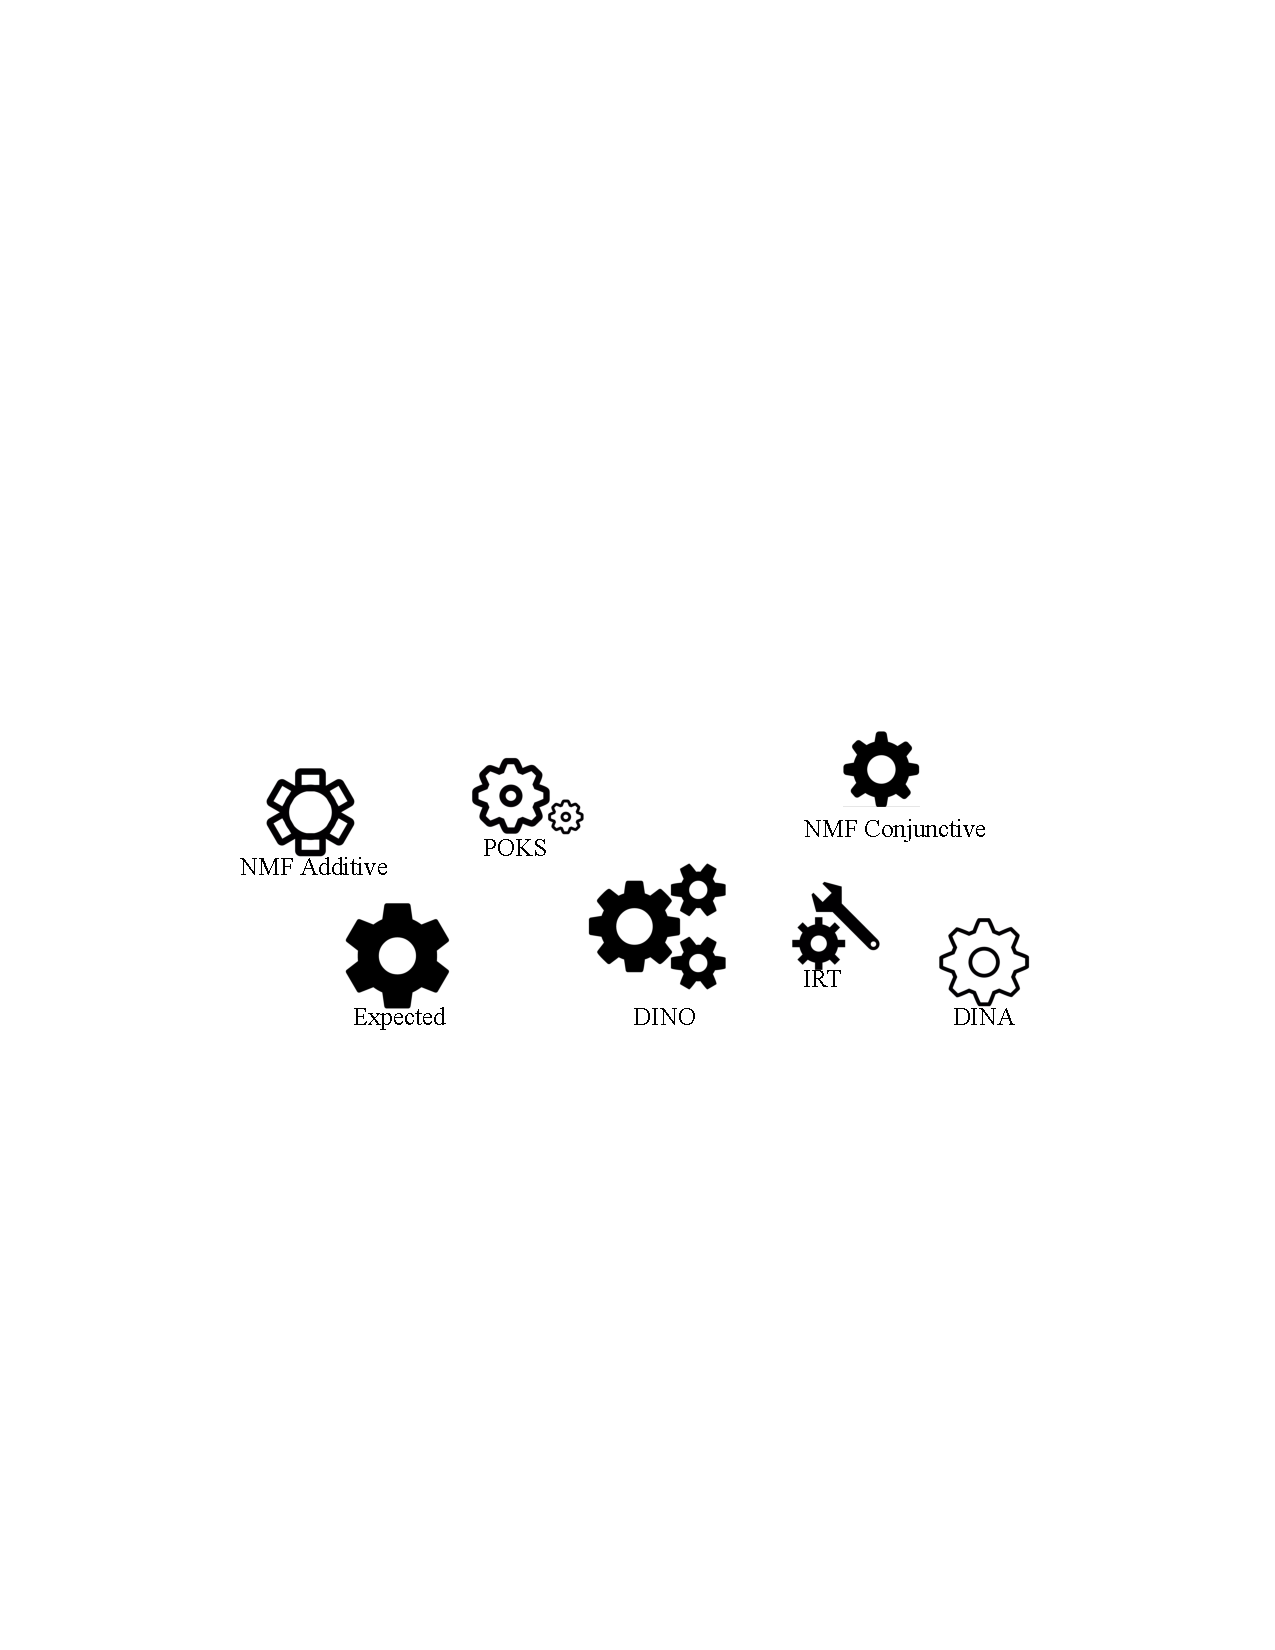
\includegraphics[trim= 0cm 6cm 0cm 8cm ,clip = true,scale =0.6]{images/Models}
      	\onslide<2> 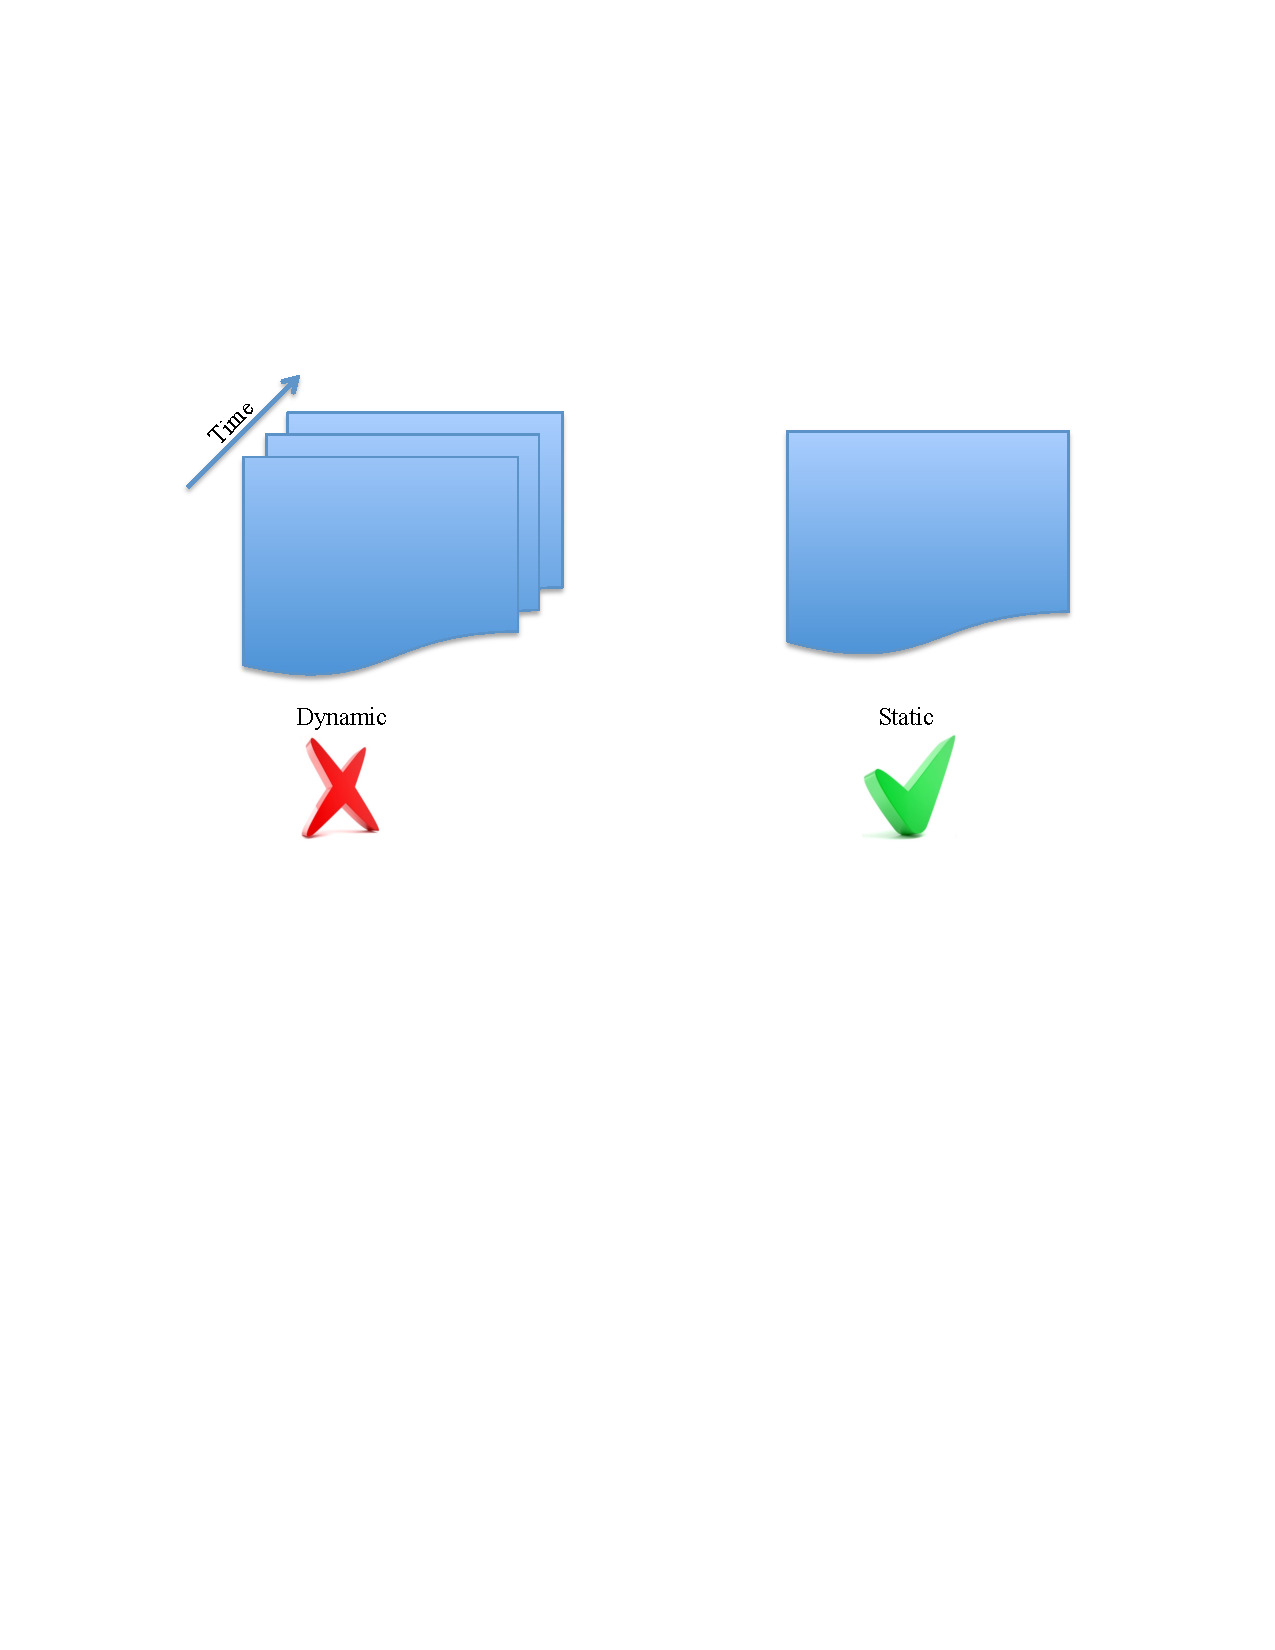
\includegraphics[trim= 0cm 5cm 0cm 0cm , scale =0.5]{images/Dynamic-Syn}
      \onslide<3> 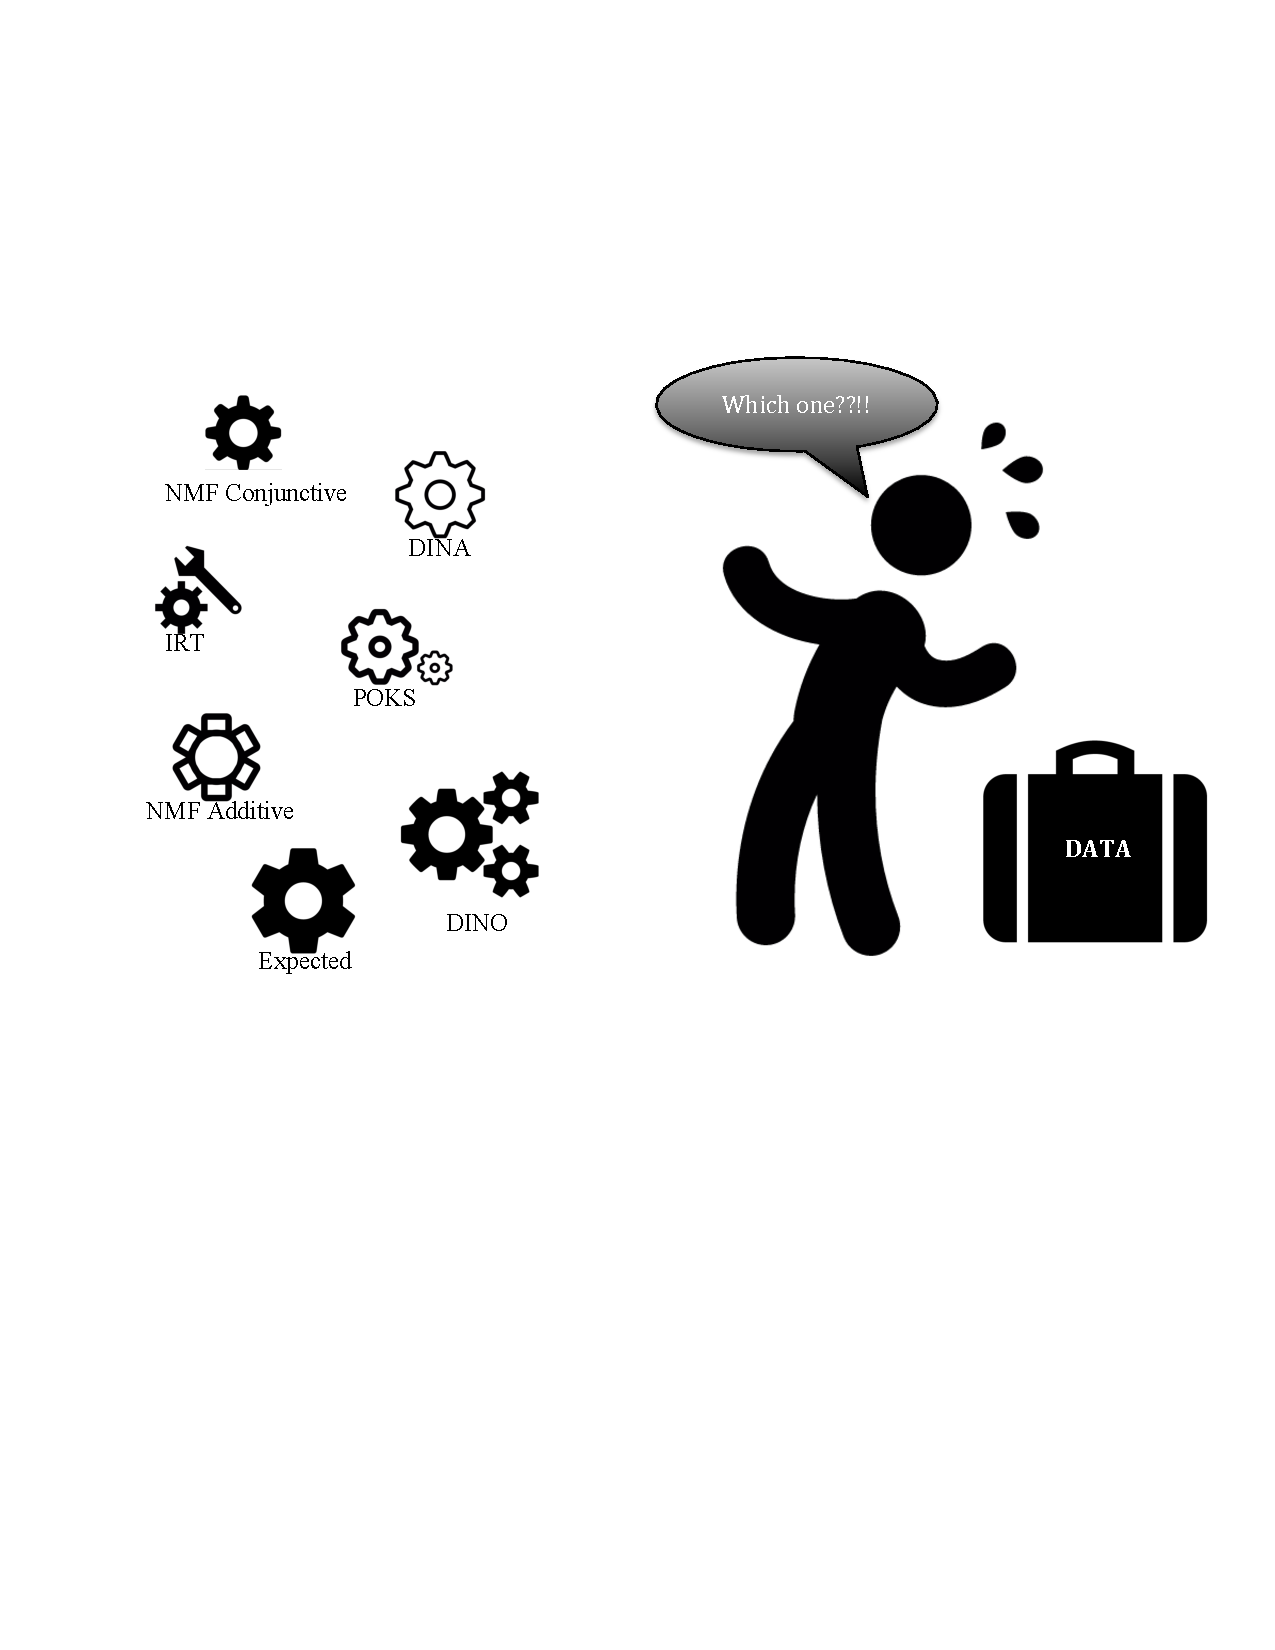
\includegraphics[trim= 0cm 0cm 0cm -3cm , scale =0.4]{images/Model-Selection}
      \onslide<4> 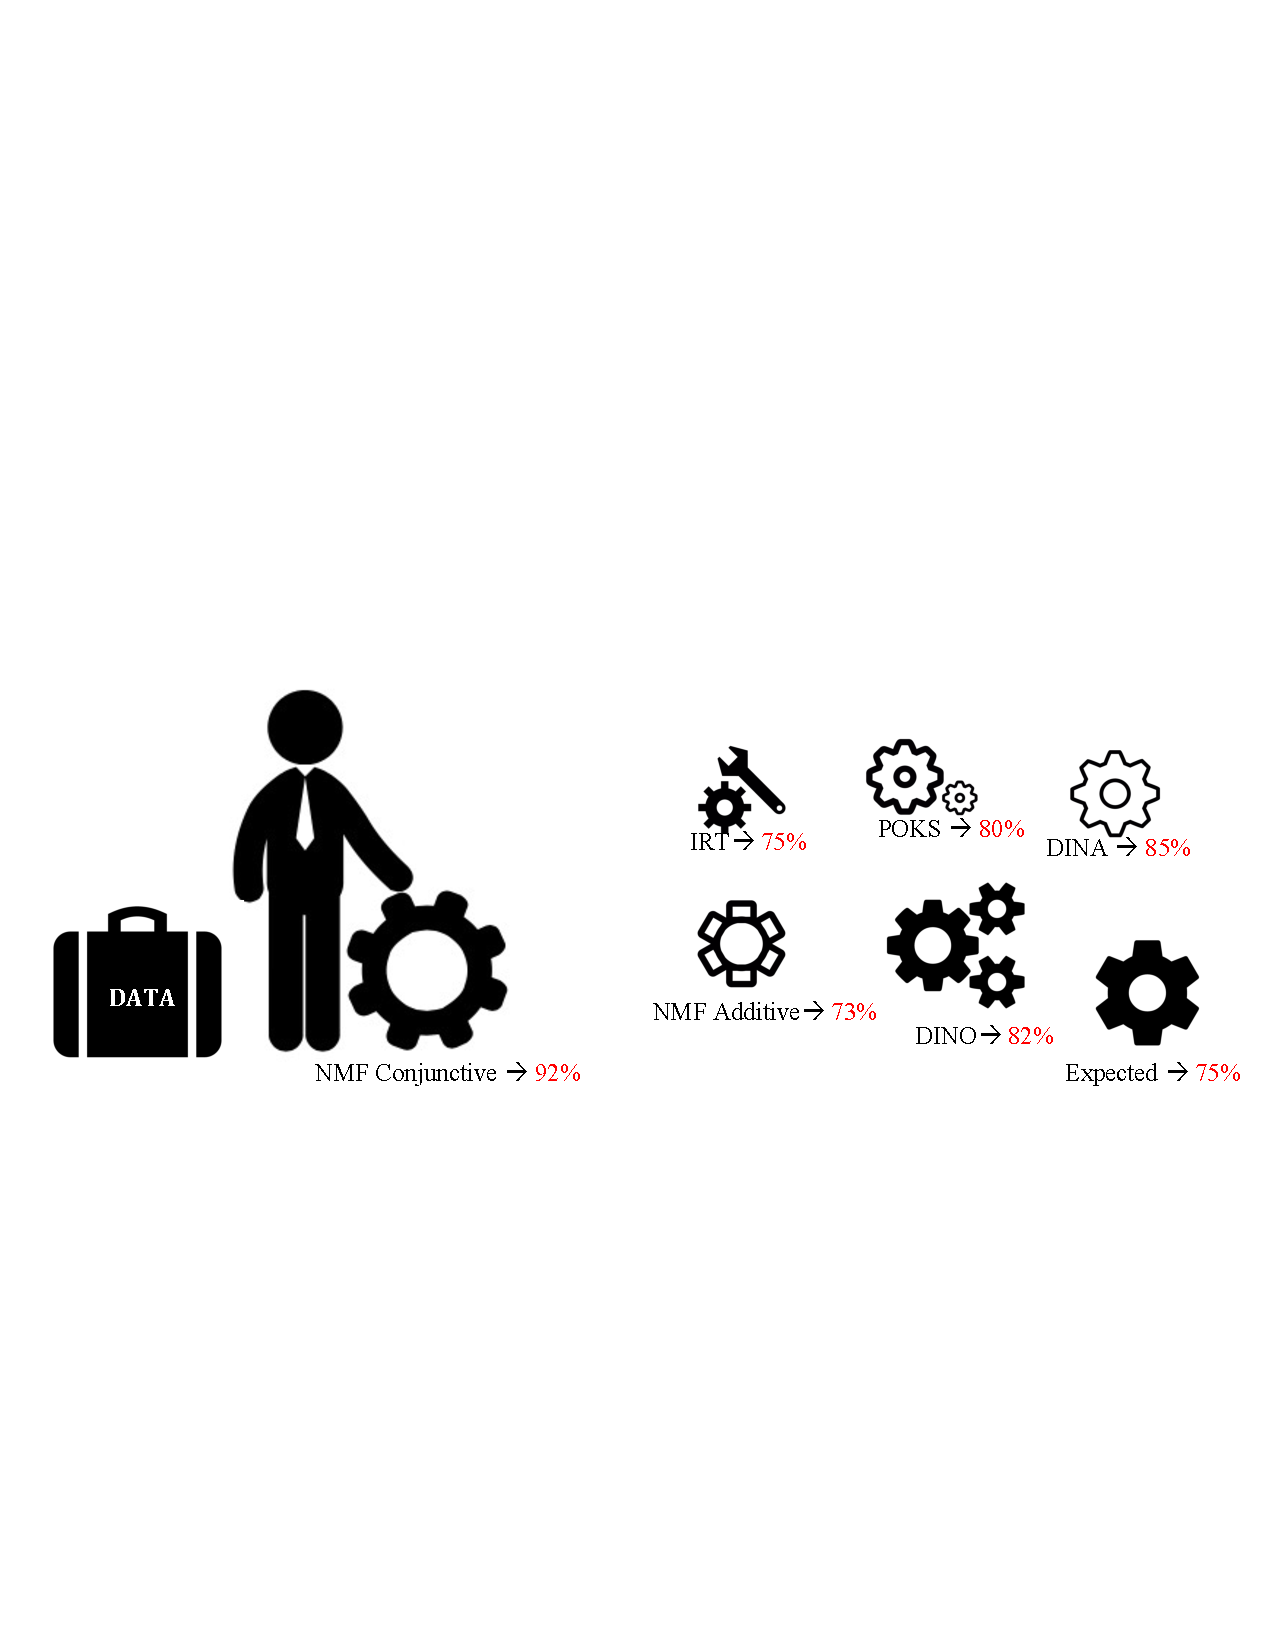
\includegraphics[trim= 0cm 5cm 0cm 2.5cm , scale =0.5]{images/Model-Selected}
%\includegraphics<2>[trim= 0cm 5cm 0cm 0cm , scale =0.5]{images/Dynamic-Syn}
%\includegraphics<3>[trim= 0cm 7cm 0cm 0cm , scale =0.4]{images/Model-Selection}
%\includegraphics<4>[trim= 0cm 5cm 0cm 2cm , scale =0.5]{images/Model-Selected}
\end{overprint}
\end{frame}

\subsection{Our approach}
\begin{frame}\frametitle{Problem Specification}
Our contribution
\begin{itemize}
\item To make a comprehensive comparison of educational data model performances
\item To propose a new approach to assessing model fit \pause
\end{itemize}
General hypothesis:
\begin{itemize}
\item Recognizing the ground truth based on the uniqueness of this comprehensive comparison \pause
\end{itemize}
The proposed approach:
\begin{itemize}
\item Assessing the fit of the model to the underlying ground truth using a methodology based on \textbf{synthetic data} 
\end{itemize}
\end{frame}

\begin{comment}
\subsection{Introduction}
\begin{frame}
\vspace{-1cm}
    \begin{block}{Student skills assessment models}
    \vspace{-0.5cm}
\resizebox{.9\columnwidth}{4cm}{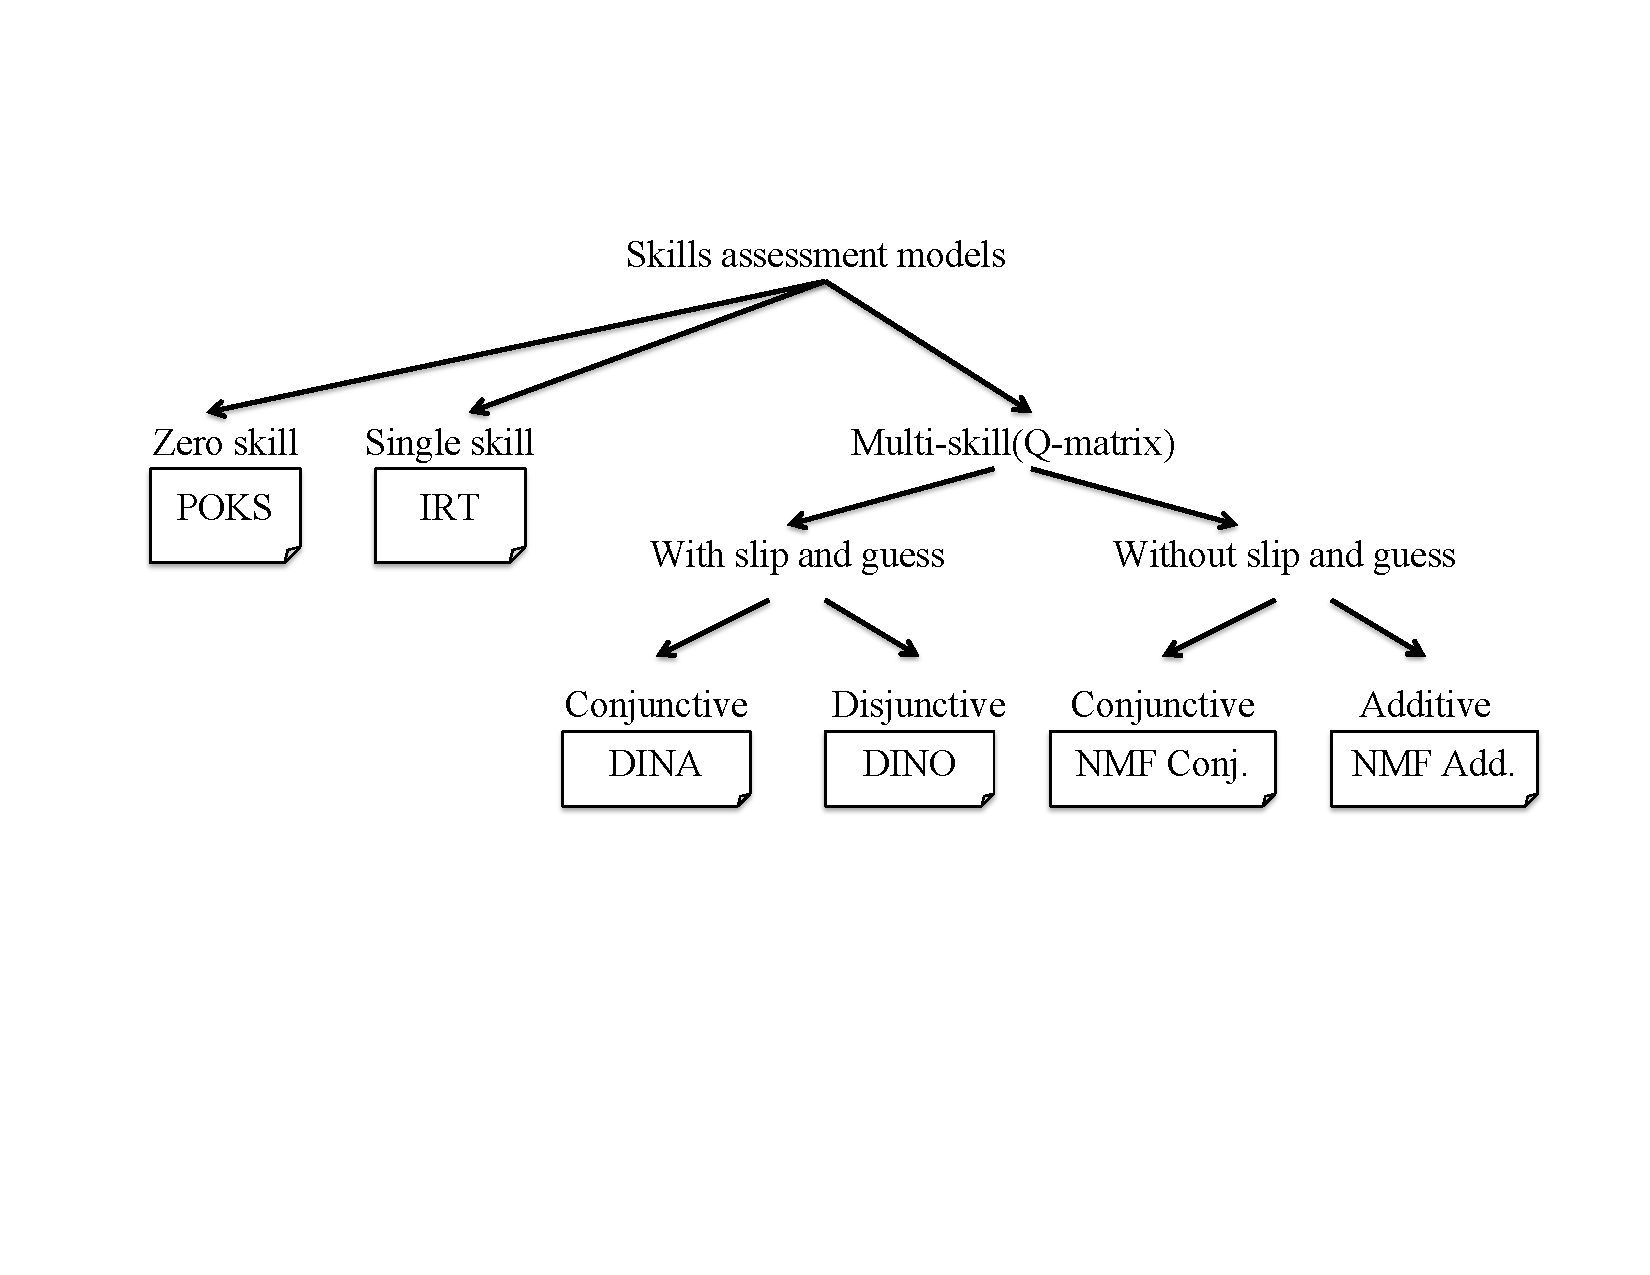
\includegraphics[trim=0.5cm 7cm 0.5cm 3cm,scale =0.4] {images/SkillsAssessments}}
    \end{block}
\begin{overprint}
      \onslide<1>
		\begin{columns}
		\begin{column}{0.35\textwidth}
      		\begin{itemize}
      		\vspace{-0.05cm}
      			\item Number of Skills
	      	\end{itemize}
	      \end{column}
	      \begin{column}{0.7\textwidth}
	      \end{column}
	     \end{columns}
      \onslide<2>
		\begin{columns}
		\begin{column}{0.35\textwidth}
      		\begin{itemize}
      		   	\vspace{-1.1cm}
      			\item Number of Skills
      			\item Q-matrix
	      	\end{itemize}
	      \end{column}
	      \begin{column}{0.7\textwidth}
	      
	      \resizebox{\columnwidth}{1.2cm}{
$\begin{array}{c|c|c}
   \begin{array}{cl}
   &\\
   &\\
   s_{1} : & \text{fraction multiplication}\\
   &\\
   s_{2} : & \text{fraction addition}\\
   &\\
   s_{3} : & \text{fraction reduction}\\
   &\\
   &
\end{array}
&
   \begin{array}{cc}
i_{1} & \frac{4}{\frac{12}{3}}+\frac{3}{5}=\frac{8}{5}\\
 &  \\
i_{2} & \frac{4}{\frac{12}{3}}=\frac{4{\times}3}{12}=\frac{12}{12}=1\\
 &  \\
i_{3} & 1+\frac{3}{5}=\frac{8}{5}\\
 &  \\
i_{4} & 2{\times}\frac{1}{2}=1\\
&
\end{array}
&
\begin{array}{c}
\begin{array}{cc}
 & \textrm{Skills}\\
 & \begin{array}{ccc}
s_{1} & s_{2} & s_{3}\end{array}\\
\mathrm{\begin{sideways}Items\end{sideways}}\begin{array}{c}
i_{1}\\
i_{2}\\
i_{3}\\
i_{4}
\end{array} & \left[\begin{array}{ccc}
1 & 1 & 1\\
1 & 0 & 1\\
0 & 1 & 1\\
1 & 0 & 1
\end{array}\right]
\end{array}\\
\\
\\

\end{array}
\end{array}$
	      }
	      
	      \end{column}
	     \end{columns}
      \onslide<3>
		\begin{columns}
		\begin{column}{0.35\textwidth}
      		\begin{itemize}
      			\item Number of Skills
      			\item Q-matrix 
      			\item Slip and Guess
	      	\end{itemize}
	      \end{column}
	      \begin{column}{0.7\textwidth}
	      \end{column}
	     \end{columns}
	     \onslide<4>
	     		\begin{columns}
		\begin{column}{0.4\textwidth}
      		\begin{itemize}
      		      		   	\vspace{-0.5cm}
      			\item Number of Skills
      			\item \textbf{Q-matrices (types)}%some are based on matrix factorization but others have more adhoc representation
      			\item Slip and Guess
	      	\end{itemize}
	      \end{column}
	      \begin{column}{0.25\textwidth}
	      \begin{enumerate}
	      \item Conjunctive
	      \item Additive 
	      \item Disjunctive
	      \end{enumerate}
	      \end{column}
	      \begin{column}{0.4\textwidth}
	      
	      \resizebox{0.66\columnwidth}{1.2cm}{

$\begin{array}{c}
\begin{array}{cc}
 & \textrm{Skills}\\
 & \begin{array}{ccc}
s_{1} & s_{2} & s_{3}\end{array}\\
\mathrm{\begin{sideways}Items\end{sideways}}\begin{array}{c}
i_{1}\\
i_{2}\\
i_{3}\\
i_{4}
\end{array} & \left[\begin{array}{ccc}
1 & 1 & 1\\
1 & 0 & 1\\
0 & 1 & 1\\
1 & 0 & 1
\end{array}\right]
\end{array}\\
\\
\\

\end{array}$
	      }
	      
	      \end{column}
	     \end{columns}
\end{overprint}
\end{frame}
\end{comment}

\newcommand{\tabitem}{~~\llap{\textbullet}~~}
\newcommand\VRule[1][\arrayrulewidth]{\vrule width #1}


\subsection{Presentation terms and concepts}
\begin{frame}\frametitle{Presentation terms and concepts}
\begin{itemize}
\item<1-> \textbf{Performance of a model} over a data set
\item<2-> Model parameters
\item<3-> Performance vector
\item<3-> Performance signature
\item<4-> Performance prototype
\item<5-> Target performance vector
\end{itemize}
\begin{overprint}
\vspace{-2cm}
\onslide<1> \centering 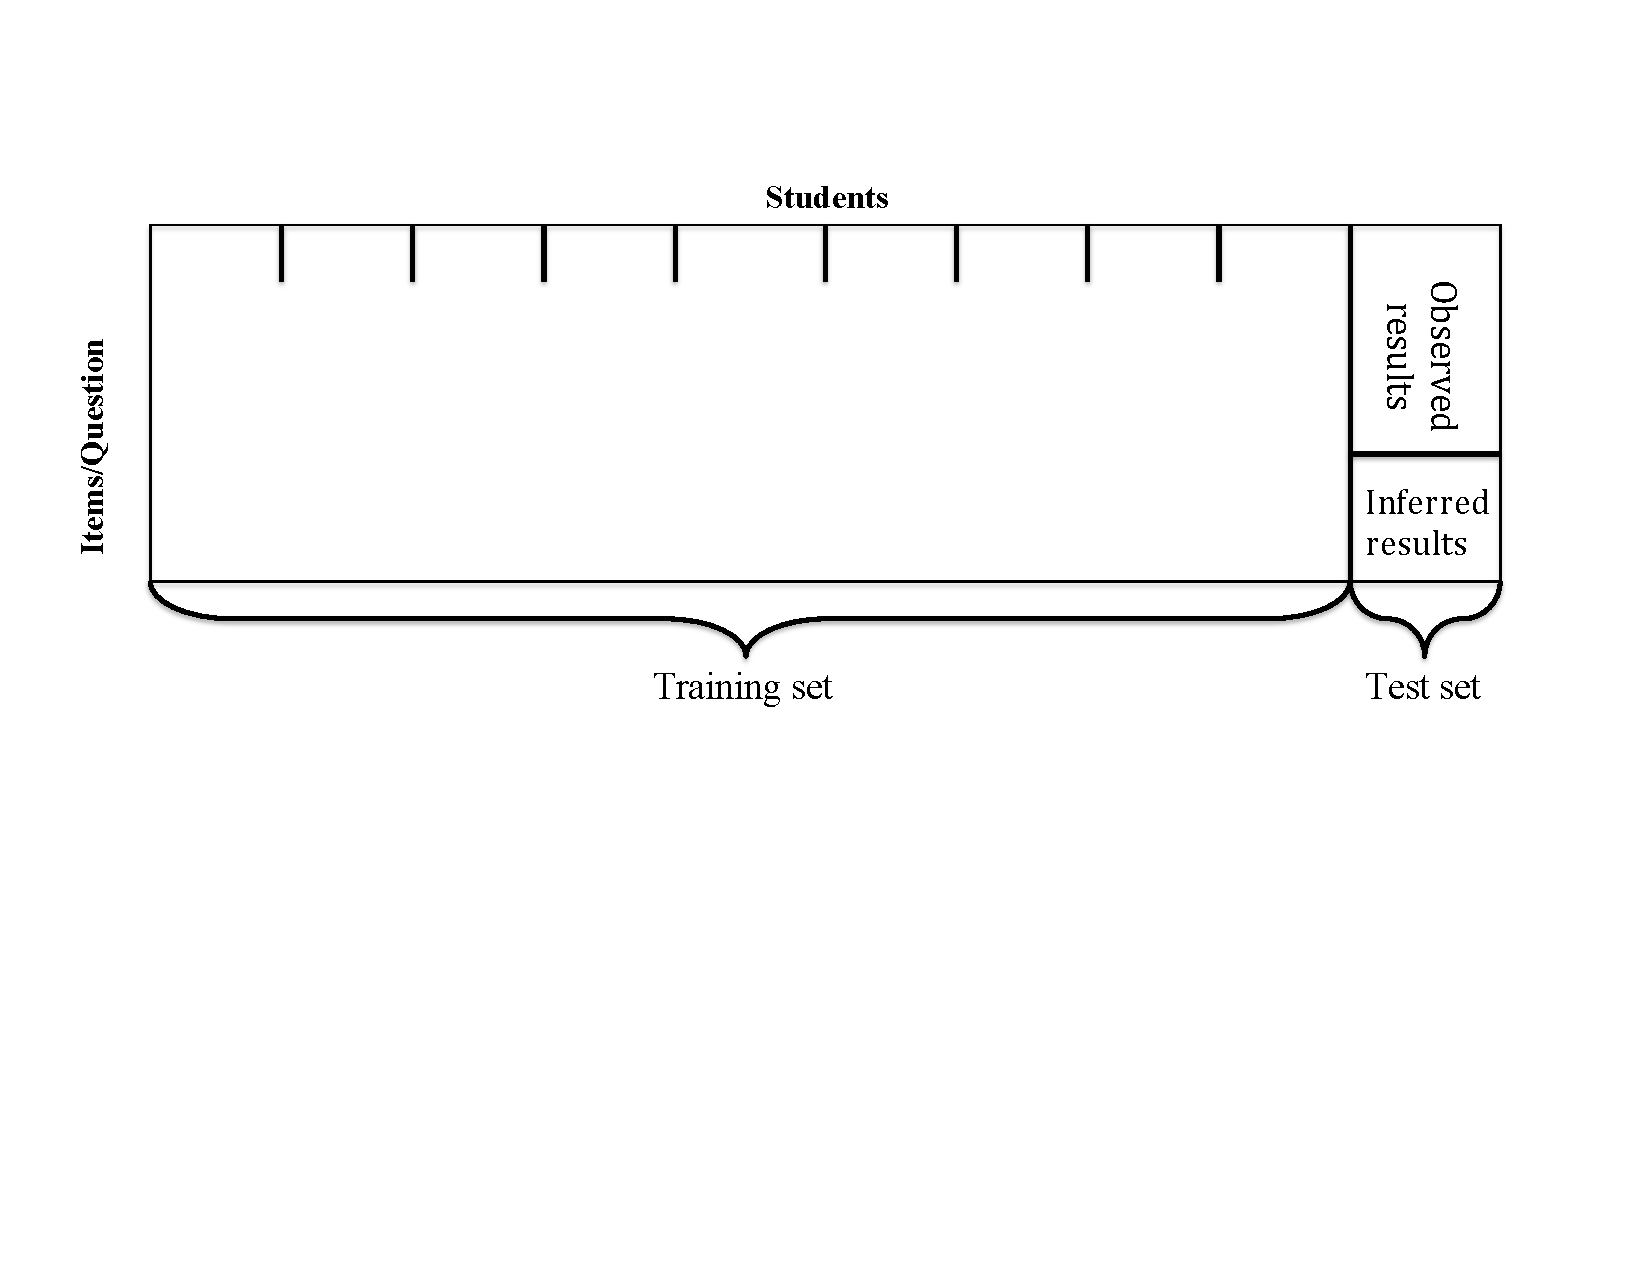
\includegraphics[trim=0cm 8.5cm 2.4cm 2.4cm,clip=true,width=\textwidth]{images/Methodology.pdf}
\onslide<2> \vspace{1cm} \centering 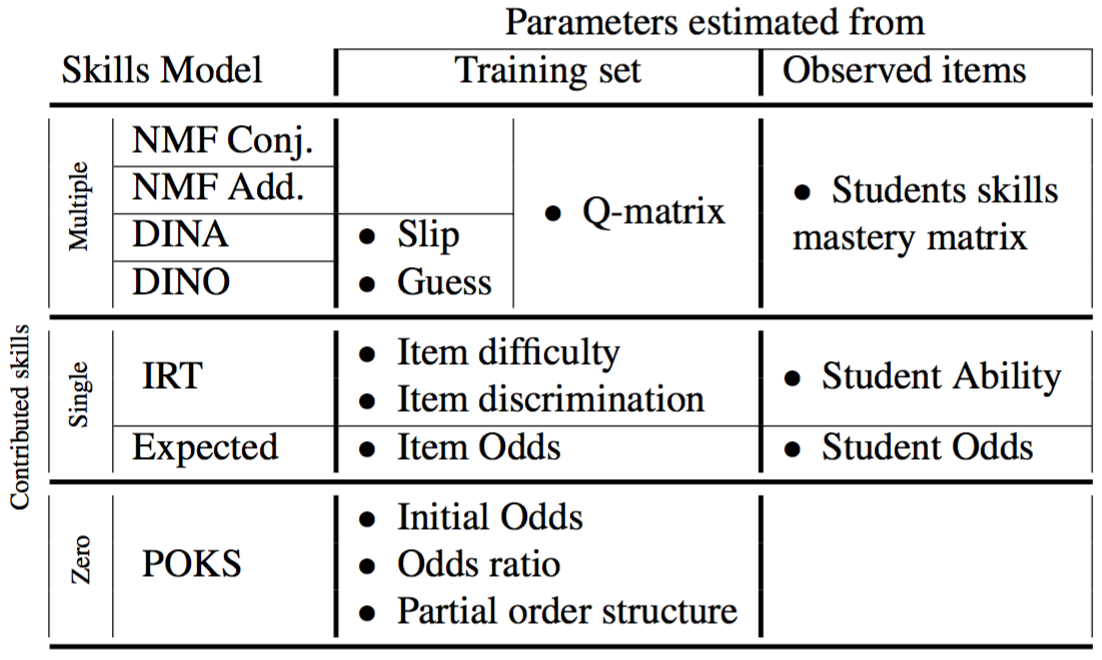
\includegraphics[width=.7\textwidth]{images/Parameters-Model}
\onslide<3>
		\begin{columns}
		\begin{column}{0.5\textwidth}
		 %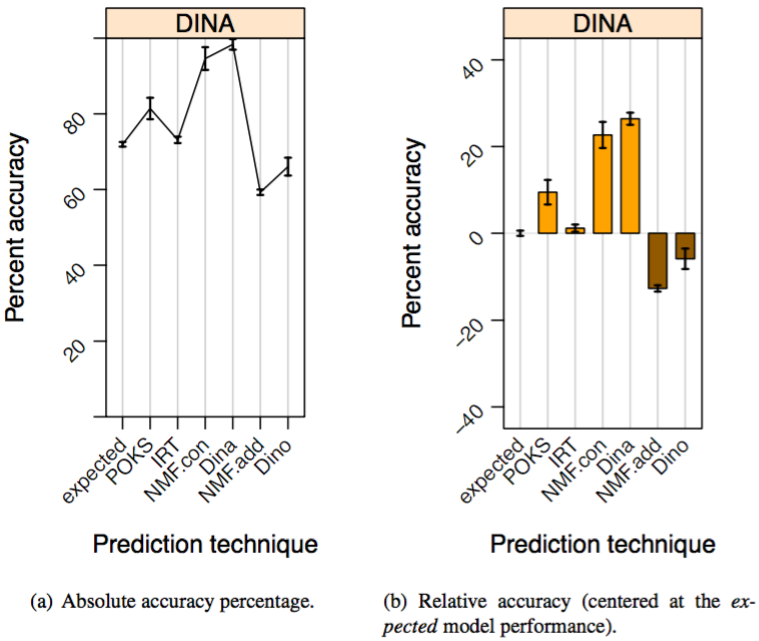
\includegraphics[trim=0cm 0cm 0cm 0cm,clip=true,width=\textwidth]{images/Performance-Presentation}	   
		 \vspace{1.25cm}   
   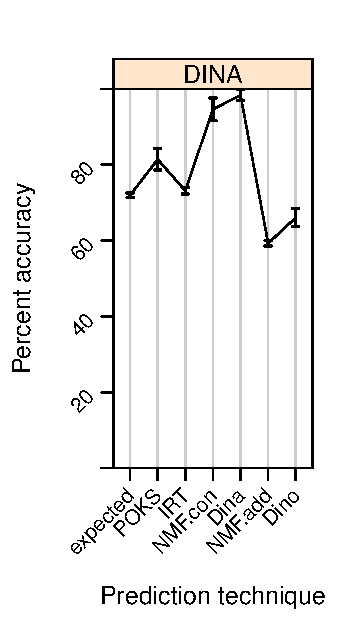
\includegraphics[trim=0cm 0cm 0cm 1.5cm,clip=true,scale =0.55] {images/Predictive-Preformace_Sig.pdf}
   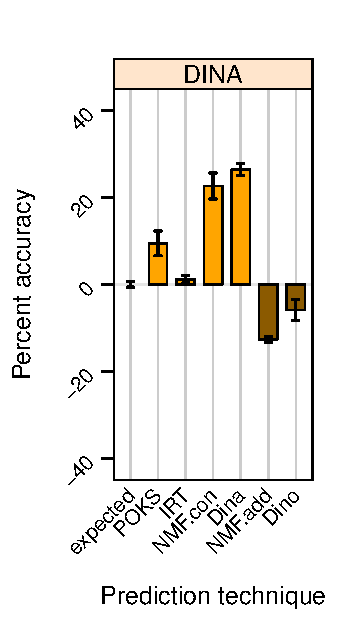
\includegraphics[trim=0cm 0cm 0cm 1.5cm,clip=true,scale =0.55] {images/Predictive-Preformace_Base.pdf}

		 \end{column}
	      \begin{column}{0.5\textwidth}
	      \[\begin{array}{l|c}
	      Model & Performace\\
	      \cline{1-2}
			Expected & 0.72\%\\
			POKS & 0.80\%\\
			IRT & 0.74\%\\
			NMF.Conj & 0.94\%\\
			Dina & 0.99\%\\
			NMF.Add & 0.60\%\\
			Dino & 0.65\%
			\end{array}
			\]
	      \end{column}
	     \end{columns}
\onslide<4>\vspace{3cm} The \textit{performance vector} associated with the synthetic data of a model class.
\onslide<5>\vspace{3cm} The \textit{performance vector} of the real data set to classify.
\end{overprint}
\end{frame}

\begin{frame}\frametitle{Vector space of accuracy performances}
\begin{overprint}
\onslide<1>
\begin{itemize}
\item Performance vectors of datasets in columns(Data points in a part of performance space)
\end{itemize}
\resizebox{\columnwidth}{!}{
\begin{tabular}{lcccccccc}
 \cline{1-8}
  \multicolumn{1}{c}{\multirow{2}{*}{\textbf{Model}}} & \multicolumn{7}{c}{\textbf{Synthetic data set }} &\multicolumn{1}{c}{\multirow{2}{*}{\textbf{\textcolor{white}{Target}}}} \\
  \cline{2-8}
  & \multicolumn{1}{c}{{\textit{Random}}} & \multicolumn{1}{c}{{POKS}} & \multicolumn{1}{c}{{IRT}} & \multicolumn{1}{c}{{DINA}} & \multicolumn{1}{c}{{DINO}} & \multicolumn{1}{c}{{L.Conj.}} & \multicolumn{1}{c}{{L.Comp.}} &\\ 
 \cline{1-8}
  \textit{Expected} & 0.75 & 0.91 & 0.90 & 0.72 & 0.72 & 0.78 & 0.93 &  \\ 
  POKS & 0.75 & 0.94 & 0.94 & 0.81 & 0.81 & 0.90 & 0.94  & \\ 
  IRT & 0.75 & 0.91 & 0.95 & 0.73 & 0.73 & 0.79 & 0.89  & \\ 
  DINA & 0.75 & 0.77 & 0.81 & 1.00 & 0.65 & 0.98 & 0.89 & \\ 
  DINO & 0.75 & 0.63 & 0.56 & 0.66 & 1.00 & 0.68 & 0.91 & \\ 
  NMF.Conj & 0.75& 0.59 & 0.53 & 0.95 & 0.65 & 0.97 & 0.58 & \\ 
  NMF.Comp & 0.75 & 0.76 & 0.79 & 0.59 & 0.93 & 0.70 & 0.98  &\\ 
 \cline{1-8}
\end{tabular}}
\vspace{.7cm}

The diagonal generally displays the best performance %the diagonal (in bold face, except for one, corresponding to the match between the underlying synthetic model and the model performance) generally displays the best perfor- mance since it corresponds to the alignment of the model and the ground truth behind the data.
\onslide<2>
\begin{itemize}
\item Given a target vector, we want to define which columns are the closest to the target column
\end{itemize}
\resizebox{\columnwidth}{!}{
\begin{tabular}{lcccccccc}
\cline{1-9}
  \multicolumn{1}{c}{\multirow{2}{*}{\textbf{Model}}} & \multicolumn{7}{c}{\textbf{Synthetic data set }} & \multicolumn{1}{c}{\multirow{2}{*}{\textbf{\textcolor{red}{Target}}}}\\
  \cline{2-8}
  & \multicolumn{1}{c}{{\textit{Random}}} & \multicolumn{1}{c}{{POKS}} & \multicolumn{1}{c}{{IRT}} & \multicolumn{1}{c}{{DINA}} & \multicolumn{1}{c}{{DINO}} & \multicolumn{1}{c}{{L.Conj.}} & \multicolumn{1}{c}{{L.Comp.}} &\\ 
\cline{1-9}
  \textit{Expected} & 0.75 & 0.91 & 0.90 & 0.72 & 0.72 & 0.78 & 0.93 & \textcolor{red}{0.43} \\ 
  POKS & 0.75 & 0.94 & 0.94 & 0.81 & 0.81 & 0.90 & 0.94  & \textcolor{red}{0.75}\\ 
  IRT & 0.75 & 0.91 & 0.95 & 0.73 & 0.73 & 0.79 & 0.89  & \textcolor{red}{0.68}\\ 
  DINA & 0.75 & 0.77 & 0.81 & 1.00 & 0.65 & 0.98 & 0.89  & \textcolor{red}{0.93}\\ 
  DINO & 0.75 & 0.63 & 0.56 & 0.66 & 1.00 & 0.68 & 0.91  & \textcolor{red}{0.60}\\ 
  NMF.Conj & 0.75& 0.59 & 0.53 & 0.95 & 0.65 & 0.97 & 0.58  & \textcolor{red}{0.80}\\ 
  NMF.Comp & 0.75 & 0.76 & 0.79 & 0.59 & 0.93 & 0.70 & 0.98  & \textcolor{red}{0.70}\\ 
\cline{1-9}
\end{tabular}}

\begin{itemize}
\item Our hypothesis : the similarity of vectors can indicate the nature of data 
\item The nearest neighbour in this space can be a candidate for the ground truth
\end{itemize}
\end{overprint}
\end{frame}

\section{Main contributions}
\subsection{Experiment 1: Predictive performance}
\begin{frame}\frametitle{Research questions}
\begin{enumerate}
\item \checkmark What is the \textit{performance vector} of student skills assessment models over real and over synthetic data created using the same models?
\begin{itemize}
\item Experiment 1: Predictive \textit{performance vector} of models over real and synthetic data sets
\end{itemize}
\end{enumerate}
\end{frame}


\begin{frame}\frametitle{Datasets}
\centering
\resizebox{7cm}{!}{
\centering
\footnotesize
\begin{tabular}{|l|c|c|r|r|l|}
\hline

%\rowcolor{\color[rgb]{.8,.8,.8}}
\multirow{2}{*}{Data set} & \multicolumn{3}{c|}{Number of} & {\parbox{6ex}{\center Mean\\Score}} & \multirow{2}{*}{Q-matrix}\tabularnewline
\cline{2-4} 
%\rowcolor{\color[rgb]{.8,.8,.8}}
 & Skills & Items & Students &  & \tabularnewline
\hline
\hline
%\rowcolor{\color[rgb]{.9,.9,.9}}
\multicolumn{6}{|c|}{\textit{Synthetic}}\\
\hline
\hline
1.Random & 7 & 30 & 700 &0.75& $\mathbf{Q}_{01}$\tabularnewline
\hline
2.POKS & 7 & 20 & 500 &0.50 & $\mathbf{Q}_{02}$\tabularnewline
\hline
3.IRT-2PL & 5 & 20 & 600 &0.50& $\mathbf{Q}_{03}$\tabularnewline
\hline
4.DINA & 7 & 28 & 500 &0.31& $\mathbf{Q}_5$\tabularnewline
\hline
5.DINO & 7 & 28 & 500 &0.69& $\mathbf{Q}_6$\tabularnewline
\hline
\multicolumn{6}{|l|}{Linear (Matrix factorization)}\\
\hline
6.~~~Conj. & 8 & 20 & 500 &0.24& $\mathbf{Q}_1$\tabularnewline
\hline
7.~~~Comp. & 8 & 20 & 500 &0.57& $\mathbf{Q}_1$ \tabularnewline
\hline
\hline
%\rowcolor{\color[rgb]{.9,.9,.9}}
\multicolumn{6}{|c|}{\textit{Real}}\\
\hline
\hline
8.Fraction & 8 & 20 & 536 &0.53& $\mathbf{Q}_1$\tabularnewline
\hline
9.Vomlel & 6 & 20 & 149 &0.61& $\mathbf{Q}_4$\tabularnewline
\hline
10.ECPE & 3 & 28 & 2922 &0.71& $\mathbf{Q}_3$\tabularnewline
\hline
\multicolumn{6}{|l|}{Fraction subsets and variants of $\mathbf{Q}_{1}$}\\
\hline
11.~~~1 & 5 & 15 & 536 &0.53& $\mathbf{Q}_{10}$\tabularnewline
\hline
12.~~~2/1 & 3 & 11 & 536 &0.51& $\mathbf{Q}_{11}$\tabularnewline
\hline
13.~~~2/2 & 5 & 11 & 536 &0.51& $\mathbf{Q}_{12}$\tabularnewline
\hline
14.~~~2/3 & 3 & 11 & 536 &0.51& $\mathbf{Q}_{13}$\tabularnewline
\hline
\end{tabular}}
\end{frame}

\begin{frame}\frametitle{Predictive performance of models over synthetic datasets}
\vspace{-0.5cm}
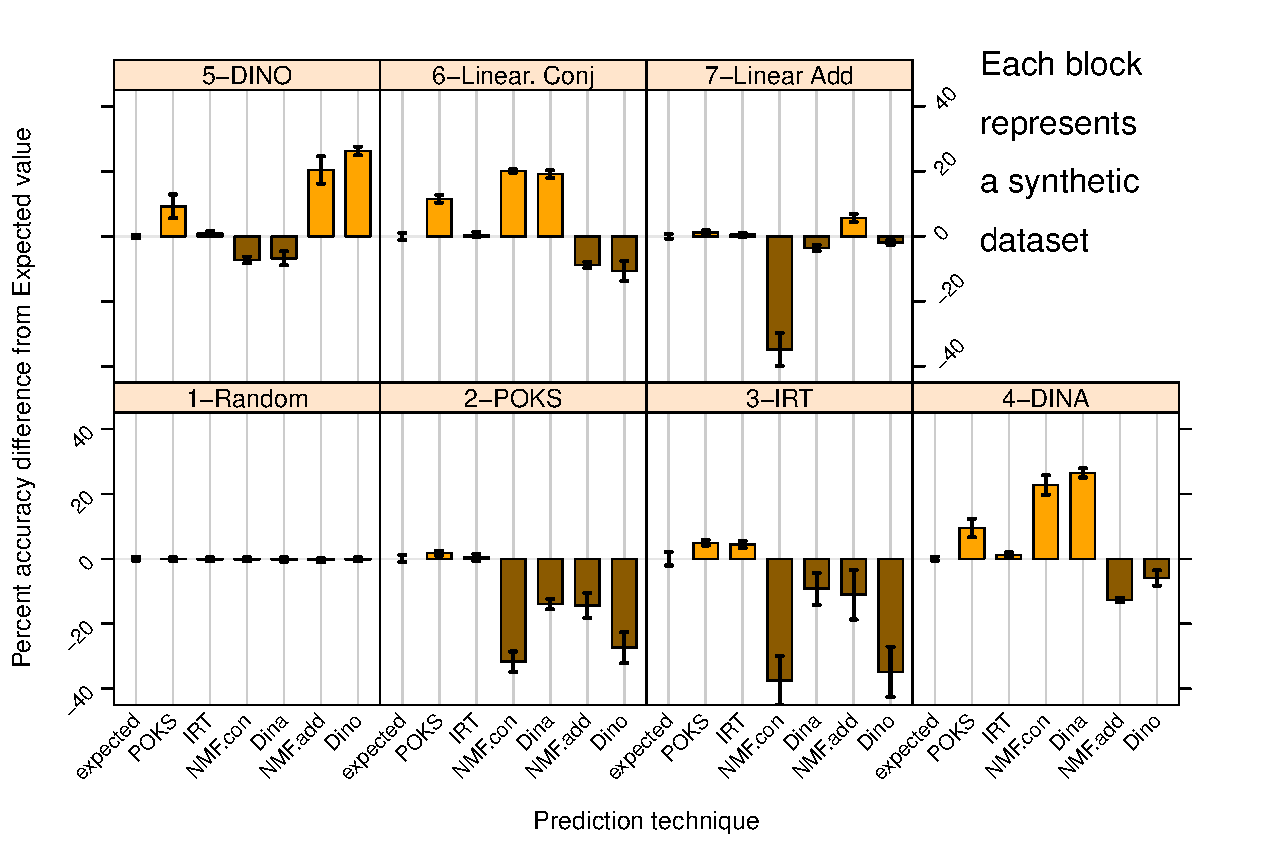
\includegraphics[scale =0.45] {images/Syn}
\begin{overprint}
     \onslide<1> The random data set has a flat performance across techniques 
     %%%which corresponds to the dominant class prediction. 
      \onslide<2> \small The highest performance is for the generative model behind the dataset
%The highest performance is for the skills assessment technique that is the same as the generative model behind the dataset%%%%the generative model behind the data set is the same as the skills assessment technique, the corresponding technique’s performance is the best, or close to the best.
	  \onslide<3> Observation: Most of the models preform worse than simple expected prediction model %You may want to point to : At first place this study was about the comparison of the models performances but it turned out that some models are doing worst than the most simple approach which is expected approach (AVG line * AVG col)
	  \onslide<4> \small Data sets have discriminant pattern of performance vector across models
	  \onslide<5> The capacity of recognizing a data set’s true model relies on this discriminant characteristic
\end{overprint}
\end{frame}

\begin{frame}\frametitle{Predictive performance of models over real datasets}
\vspace{-0.5cm}
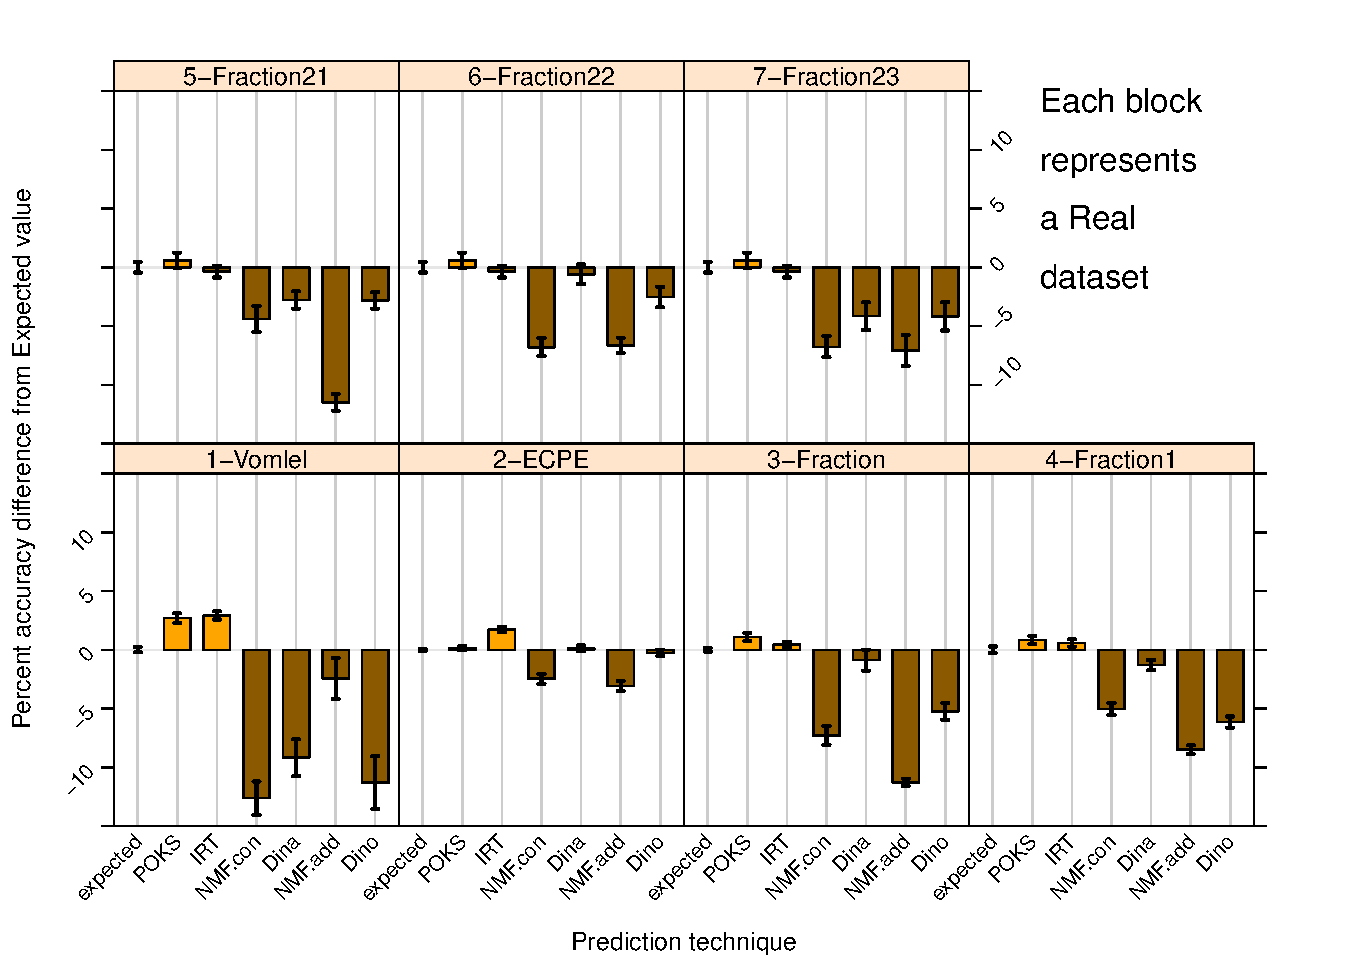
\includegraphics[scale =0.4] {images/Real}
\begin{overprint}
      \onslide<1> In most cases, the best performer is close to the baseline %many methods are not doing better than expected value
      \onslide<2> The pattern of the Fraction performance data set repeats over its subsets %Fraction-1, Fraction-2/1 and Fraction-2/2, in spite of the different number of skills and different subsets of questions
      %this similarity among Fraction data set and its derivative suggests that in spite of the model differences (different Q-matrices and item subsets), the performance signature remains constant across these data sets.
      \onslide<3> None of the real data sets show the large variance and the differences found in the synthetic data sets models %Scles are 4 times bigger
\end{overprint}
\end{frame}


\subsection{Experiment 2: Sensitivity of the Model performance}
\begin{frame}\frametitle{Research questions}
\begin{enumerate}
\item \checkmark What is the \textit{performance vector} of student skills assessment models over real and over synthetic data created using the same models?
\begin{itemize}
\item Experiment 1: Predictive performance of models over real and synthetic data sets
\end{itemize}
\item \textbf{Is the \textit{performance vector} unique to each synthetic data type (data from the same ground truth model)?}
\begin{itemize}
\item Experiment 2: Sensitivity of the Model performance over different data generation parameters
\end{itemize}
\textbf{Are they stable across the data parameter space in addition to be discriminant?}
%It’s is not only that performance is dependent to the data parameters but we wanted to check if the signature totally changes with different data parameters or it stays stable? if it changes my hypothesis will not stay anymore, and if it totally changes then the nearest neighbour or correlation would not work here.
\end{enumerate}
\end{frame}

\begin{frame}\frametitle{Variation of sample size over synthetic data sets}
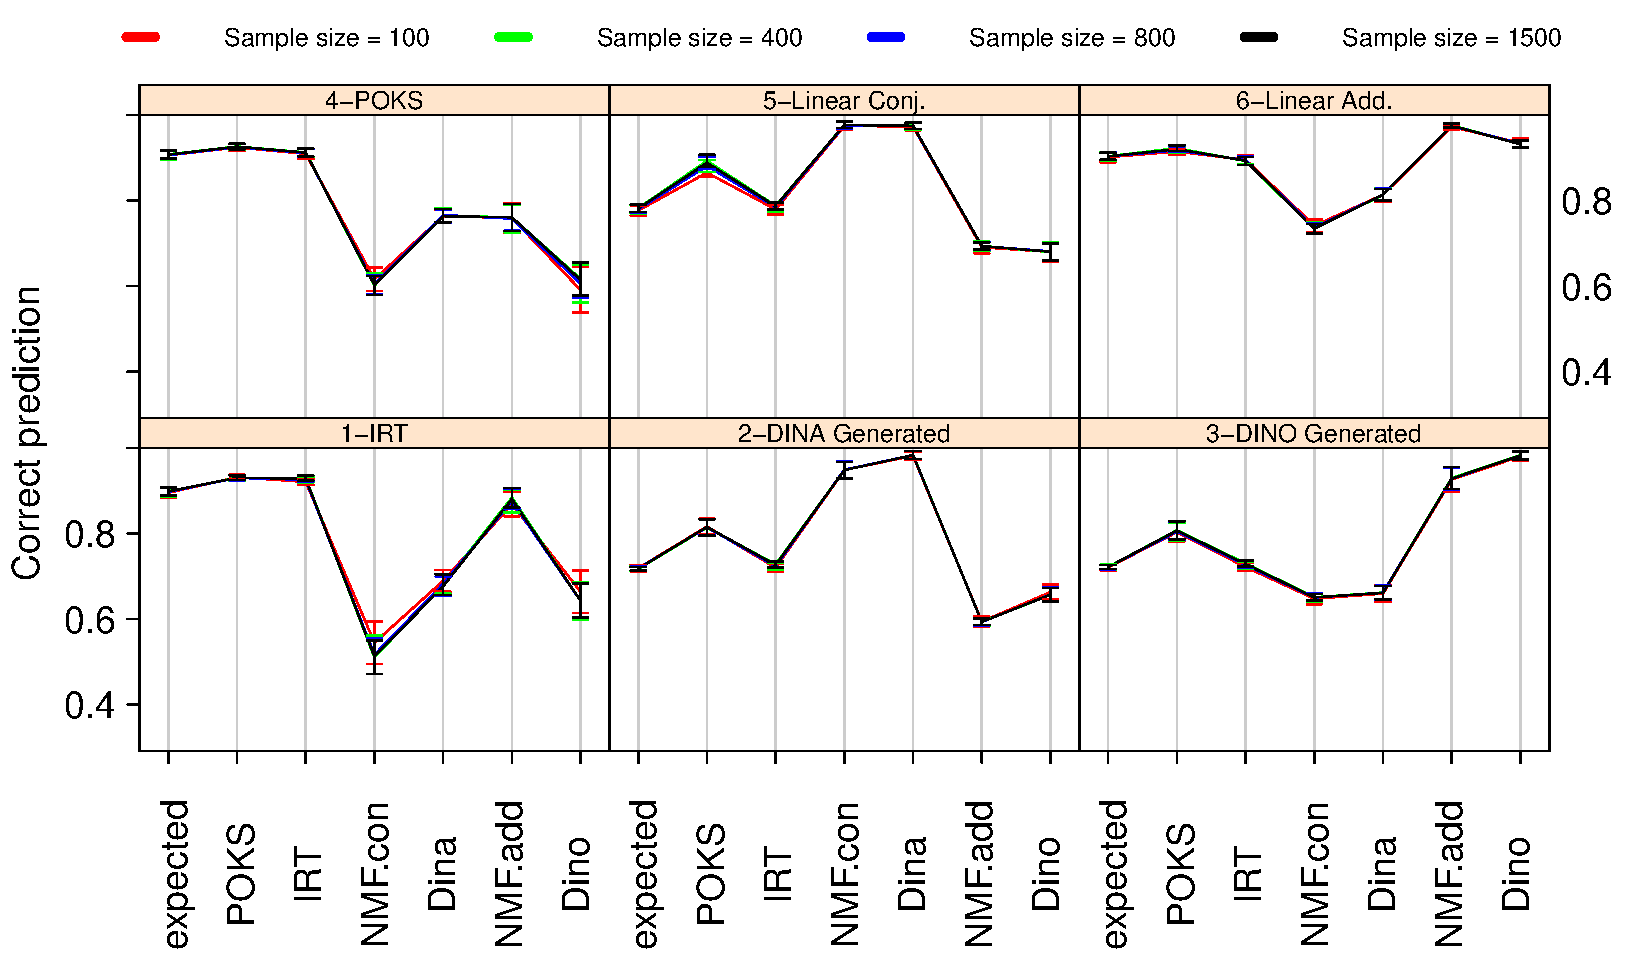
\includegraphics[scale =0.37] {images/SampleSize}
\begin{overprint}
      \onslide<1> Obviously, the signature pattern did not change significantly for some parameters such as \textbf{Sample size}.
\end{overprint}
\end{frame}

\begin{frame}\frametitle{Variation of number of items over synthetic data sets}
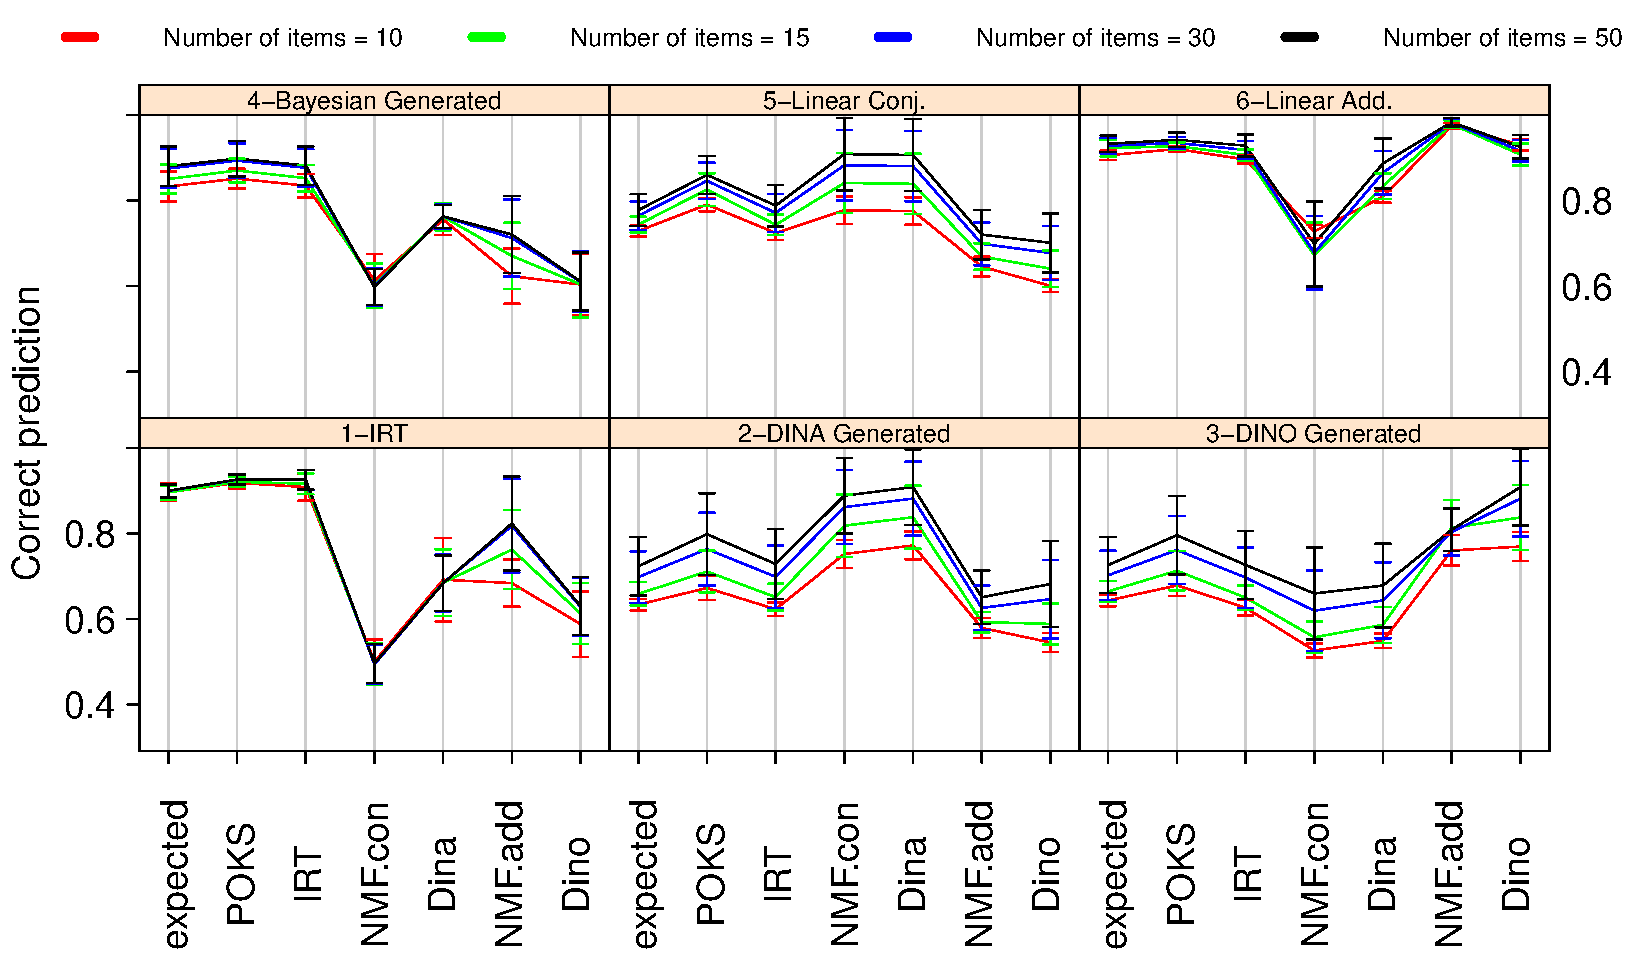
\includegraphics[scale =0.37] {images/numberofitems}
\begin{overprint}
	  \onslide<1> Even for synthetic data the performance of the ground truth model should not necessarily be close to 100\%.
      \onslide<2> The Performance signature shifts down once the number of items degrades.
\end{overprint}
\end{frame}

\begin{frame}\frametitle{Data parameters}
\begin{enumerate}
\item Sample size (Number of students)
\item Number of items
\item Number of latent skills
\item Item score variance 
\item Student score variance
\item Average success rate\pause
\end{enumerate}
Conclusion :
\begin{itemize}
      \item Data parameters can potentially influence the performance of a model%the best performer may not be the model that is most representative of the ground truth, but instead it may be the result of contextual factors that make this model outperform the ground truth one.
	  \item For better comparison of the vectors, we also consider \textbf{data characteristic parameters} of the real data in the generation process%we can also consider data specific parameters of the real data in the generation process to make a better comparison of the results.
\end{itemize}
\end{frame}

\subsection{Experiment 3: Signature Approach}
\begin{frame}\frametitle{Research questions}
\begin{enumerate}
\item \checkmark What is the \textit{performance vector} of student skills assessment models over real and over synthetic data created using the same models?
\begin{itemize}
\item Experiment 1: Predictive performance of models over real and synthetic data sets
\end{itemize}
\item \checkmark Is the \textit{performance vector} unique to each synthetic data type (data from the same ground truth model)?
\begin{itemize}
\item Experiment 2: Sensitivity of the Model performance over different data generation parameters
\end{itemize}
\item \textbf{Can the \textit{performance vector} be used to define a method to reliably identify the ground truth behind the synthetic data?}
\begin{itemize}
\item Experiment 3: Model selection based on performance vector classification
\end{itemize}
\end{enumerate}
\end{frame}

\begin{frame}\frametitle{Signature framework}
This approach relies on generating synthetic datasets
\begin{overprint}
\onslide<1> 
		\begin{columns}
		\begin{column}{0.7\textwidth}
		\vspace{-0.8cm}
			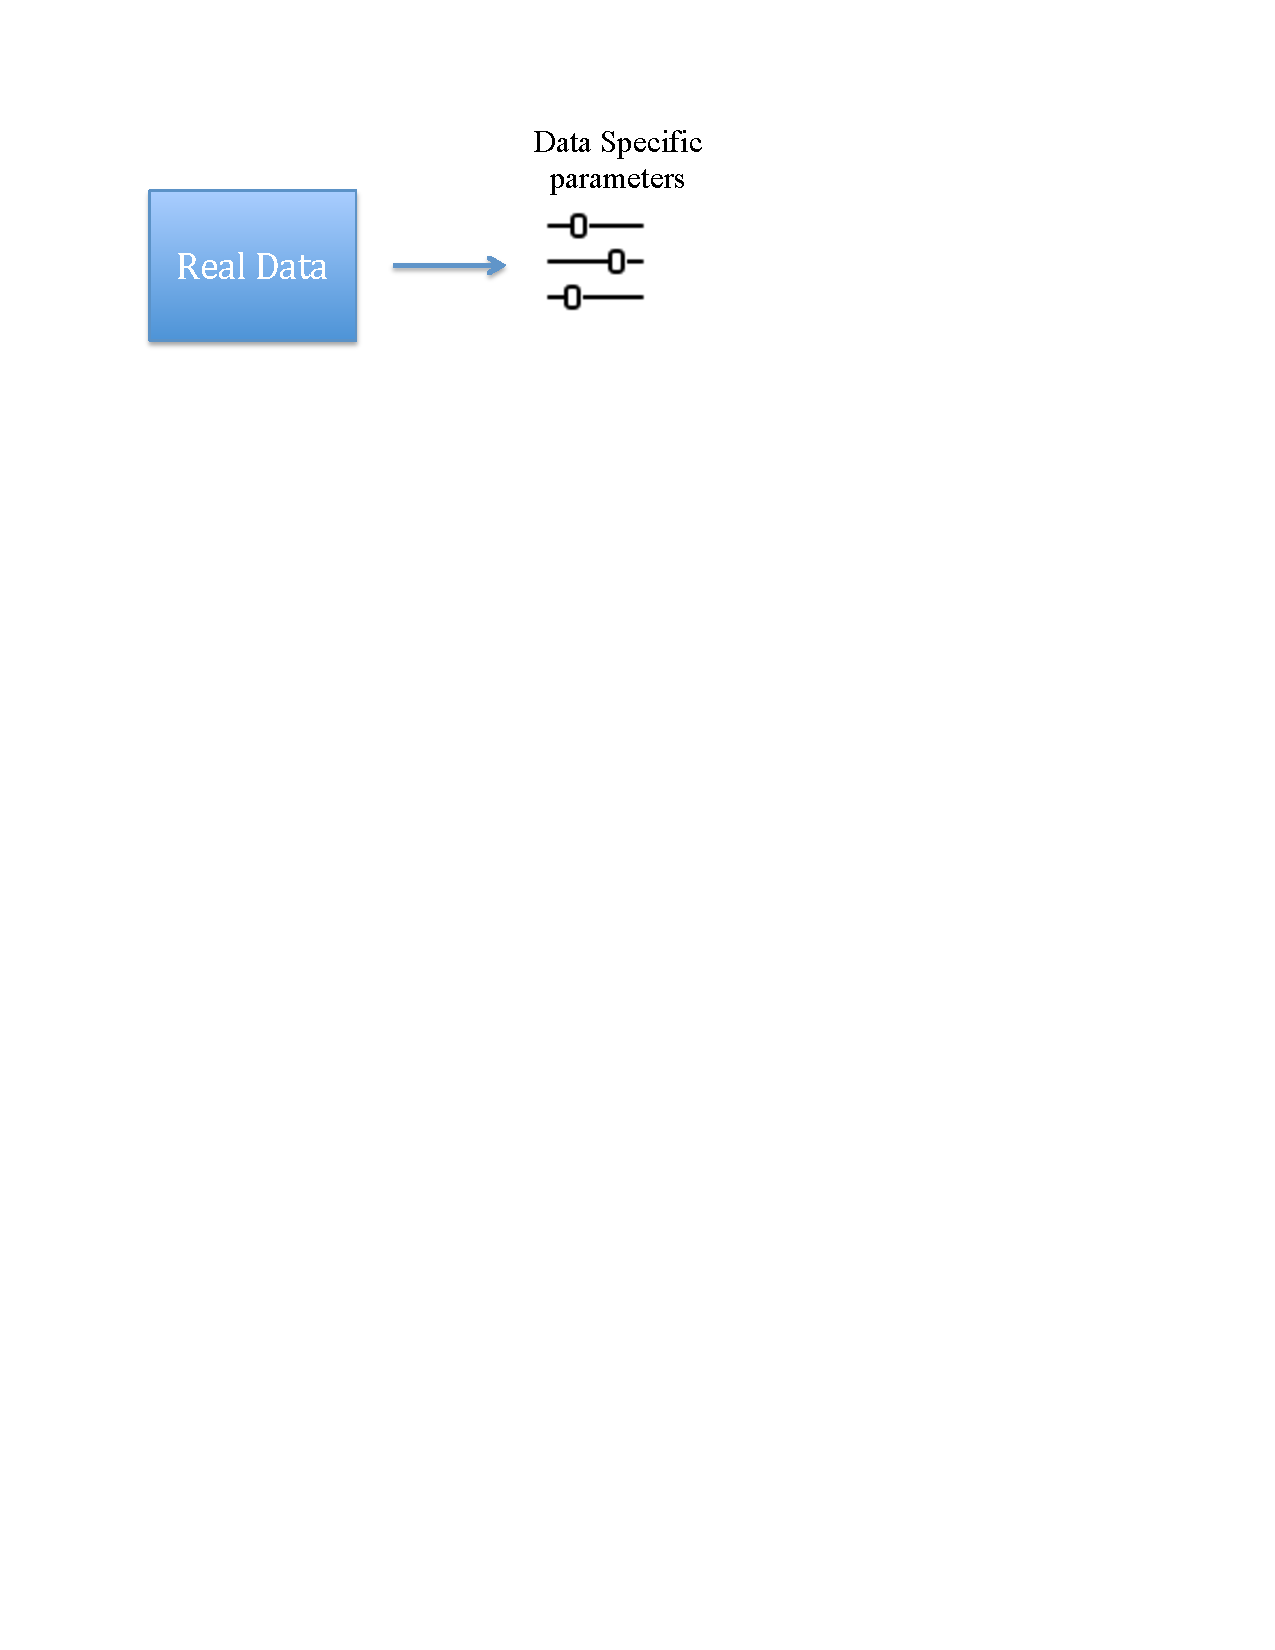
\includegraphics[trim=1cm 10cm 1cm 1cm,scale=0.43]{images/Approach1.pdf}
		\end{column}
		\begin{column}{0.3\textwidth}
		\end{column}
		\end{columns}
\onslide<2> 		\begin{columns}
		\begin{column}{0.7\textwidth}
		\vspace{-0.8cm}
			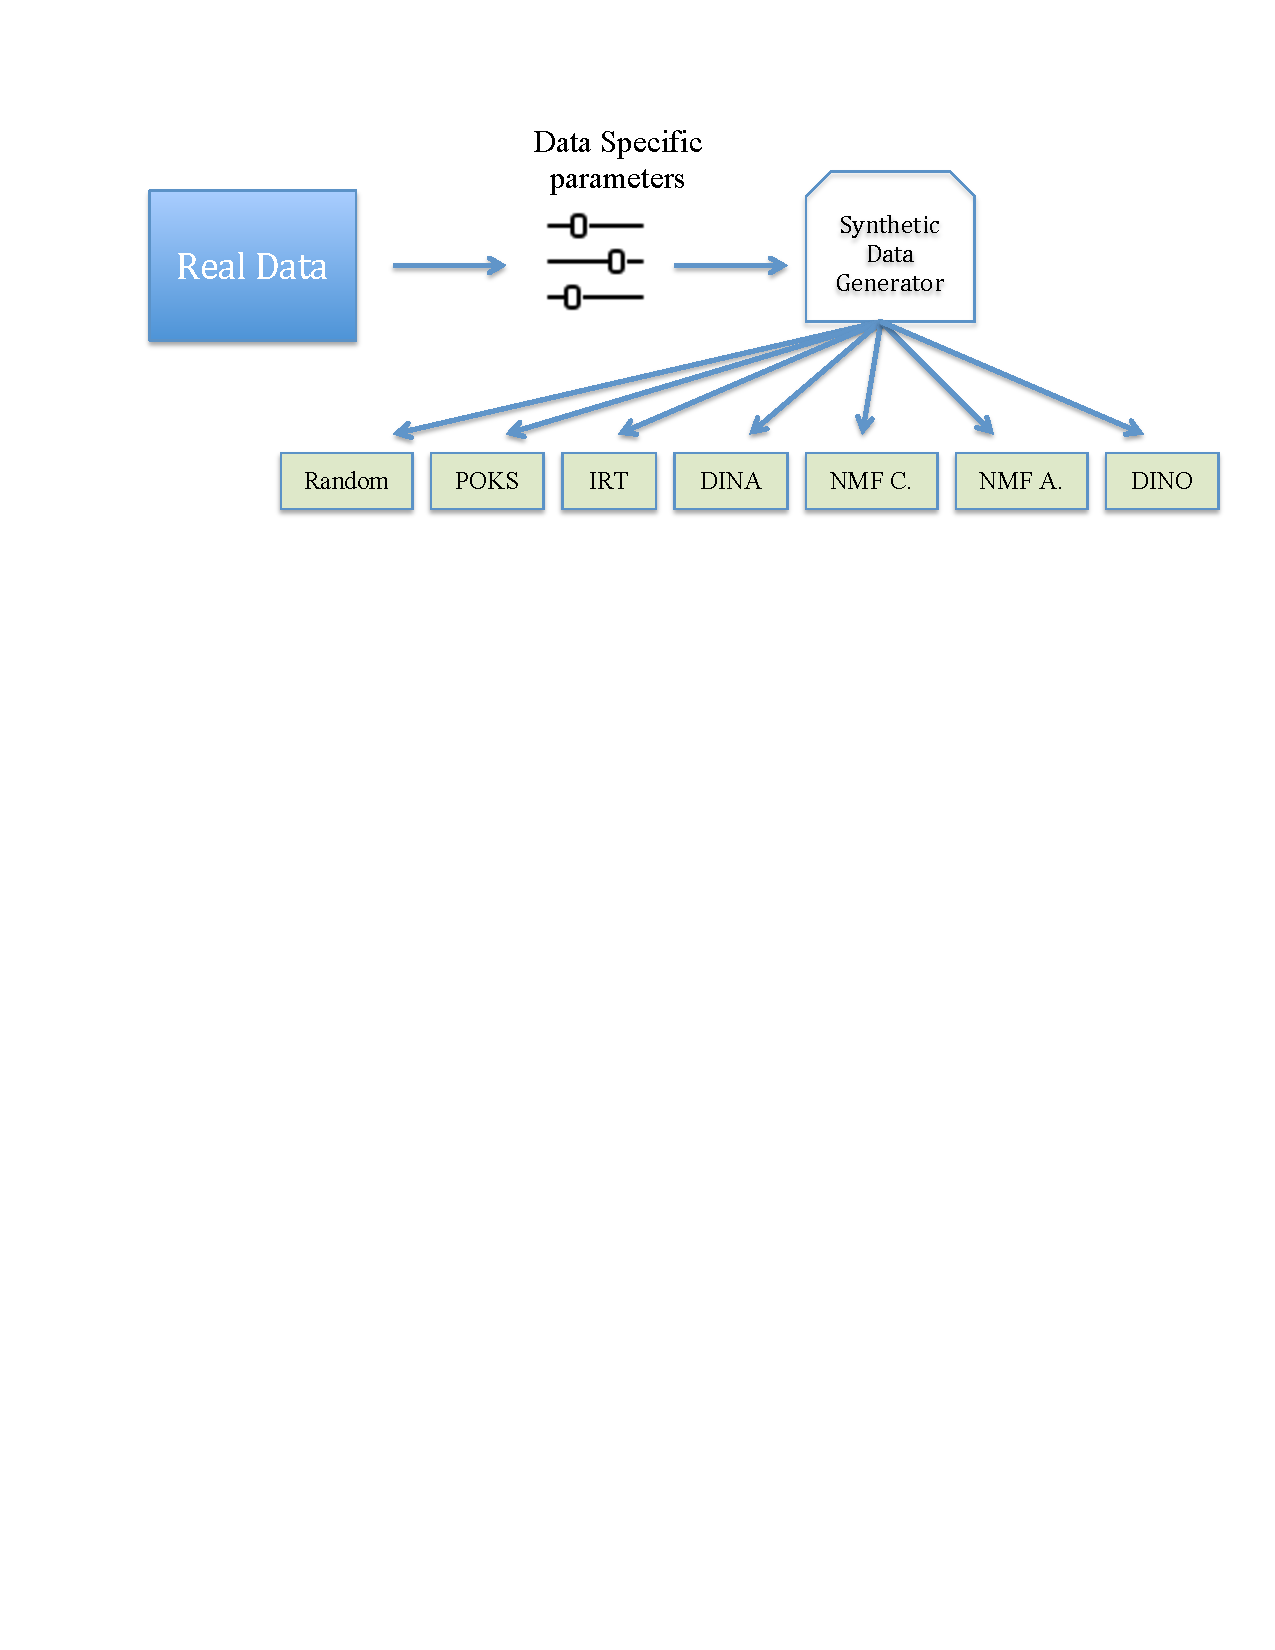
\includegraphics[trim=1cm 10cm 1cm 1cm,scale=0.43]{images/Approach2.pdf}
		\end{column}
		\begin{column}{0.3\textwidth}
		\end{column}
		\end{columns}
		\onslide<3> 		\begin{columns}
		\begin{column}{0.7\textwidth}
			\vspace{-0.8cm}
			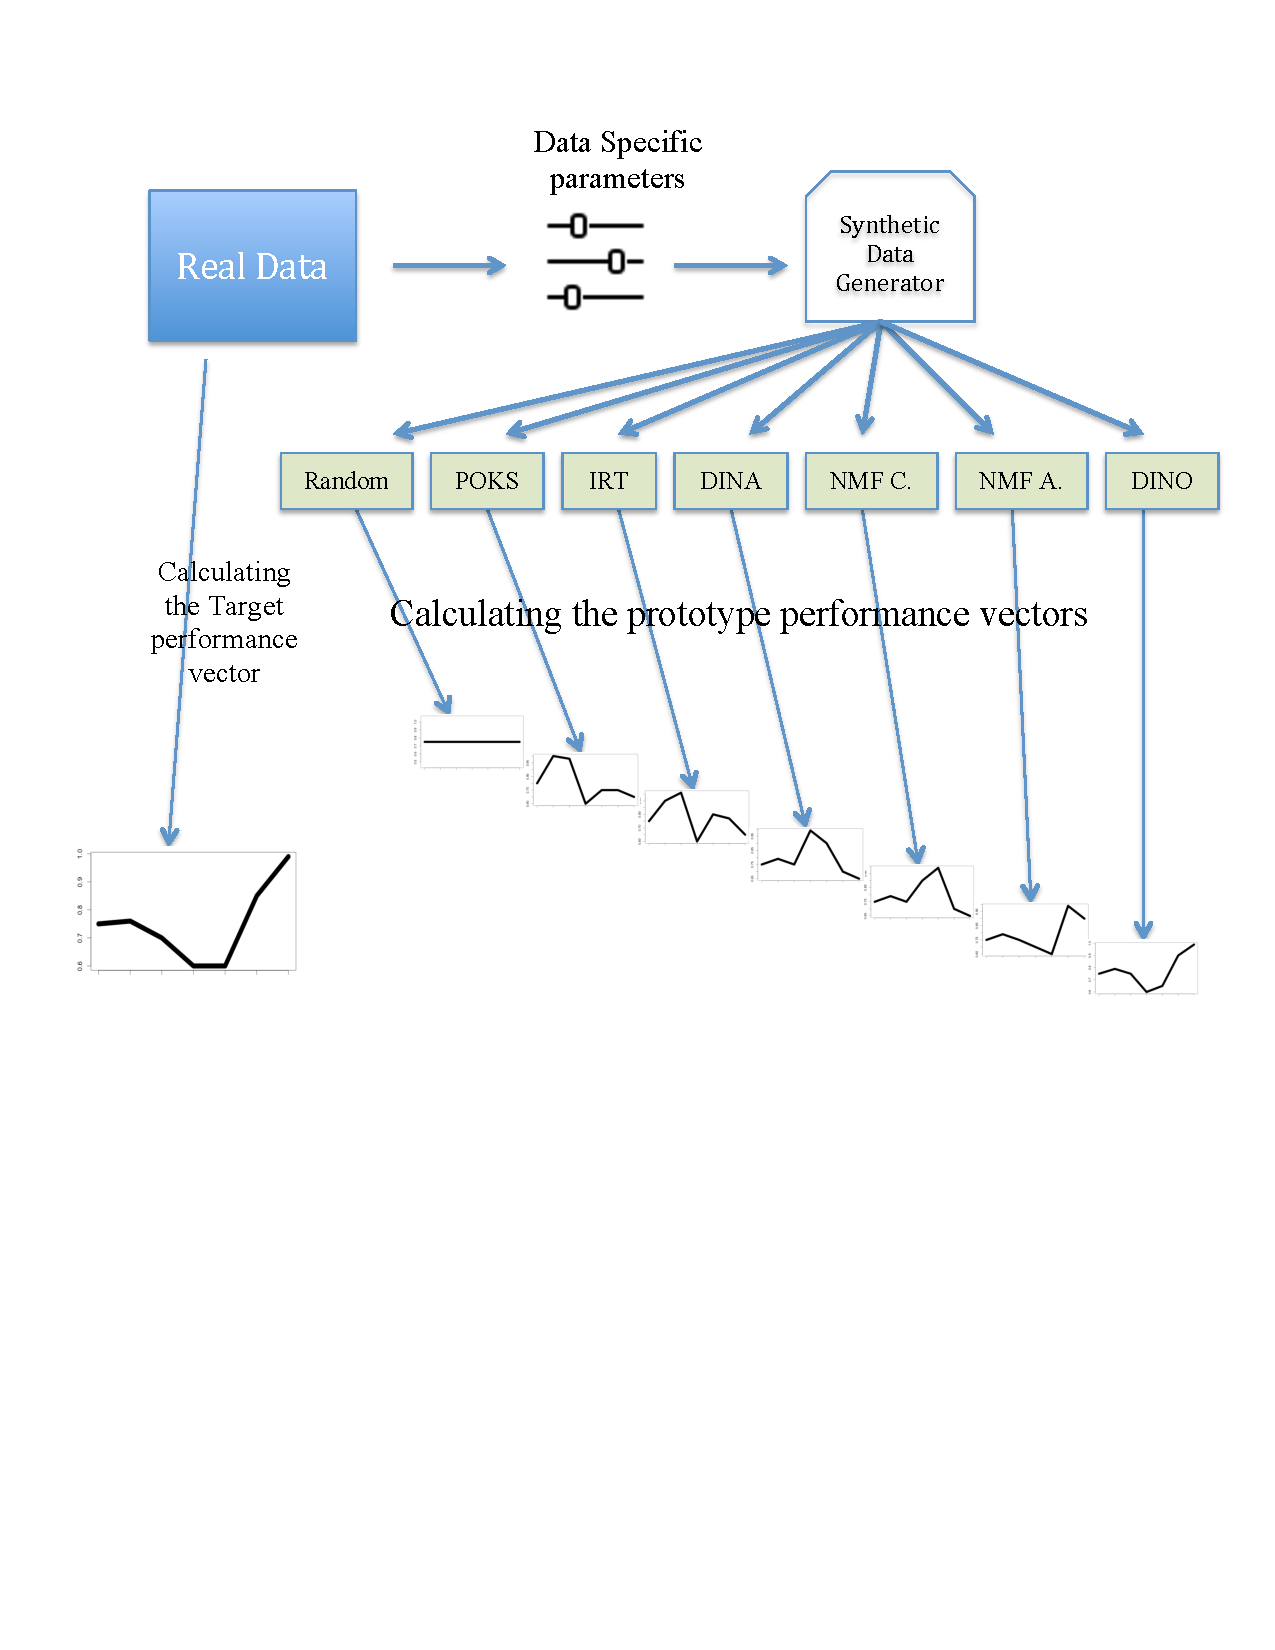
\includegraphics[trim=1cm 10cm 1cm 1cm,scale=0.43]{images/Approach3.pdf}
		\end{column}
		\begin{column}{0.3\textwidth}
			\hspace{1.5cm}Recall
          
          \vspace{1cm}
           \rightline{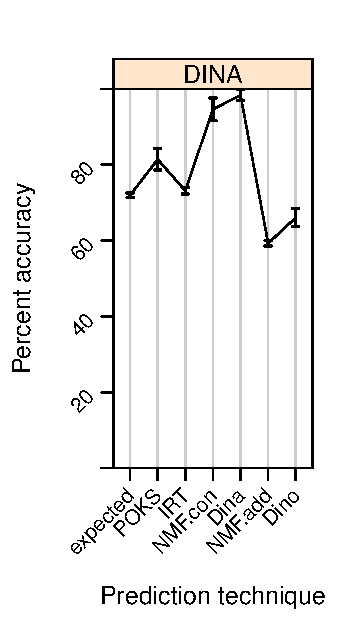
\includegraphics[trim=0cm 0cm 0cm 1.5cm,clip=true,scale =0.5] {images/Predictive-Preformace_Sig.pdf}}


		\end{column}
		\end{columns}
		\onslide<4> 		\begin{columns}
		\begin{column}{0.7\textwidth}
			\vspace{-0.8cm}			
			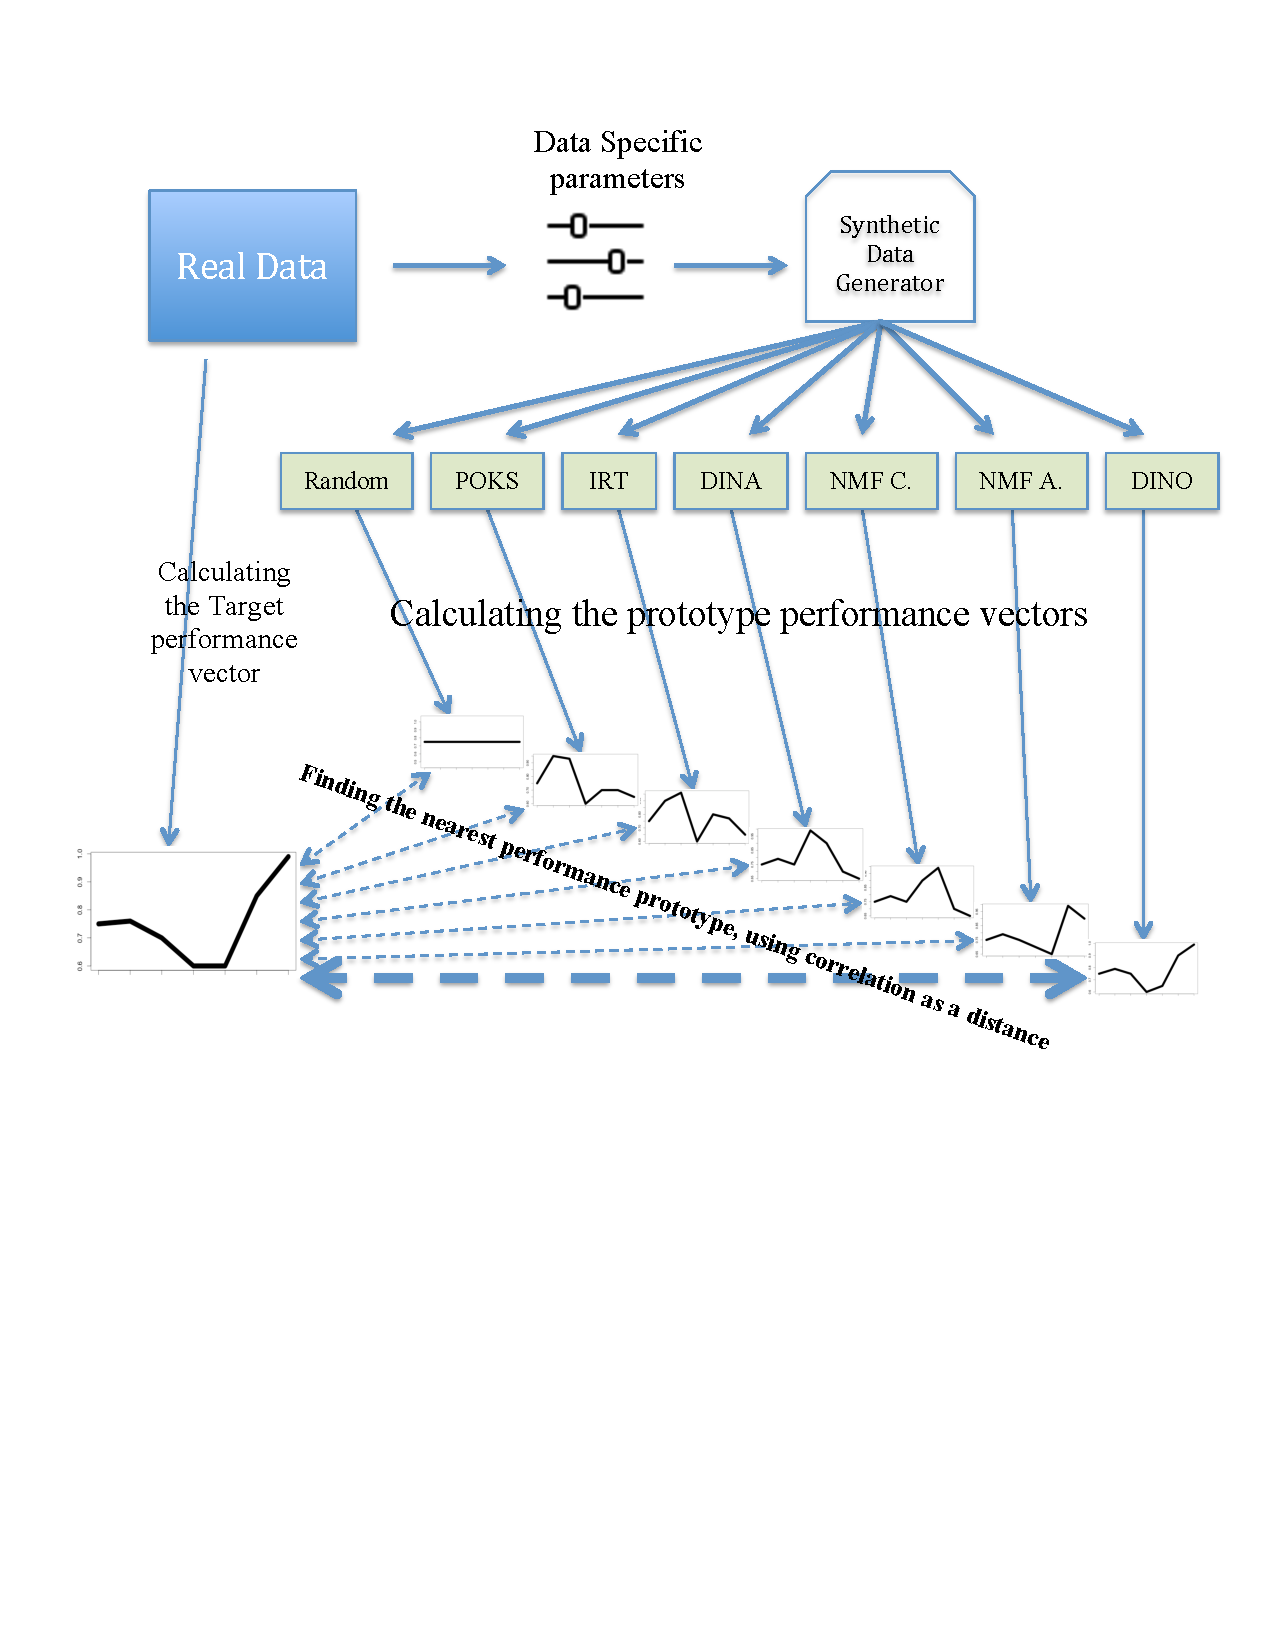
\includegraphics[trim=1cm 10cm 1cm 1cm,scale=0.43]{images/Approach4.pdf}
		\end{column}
		\begin{column}{0.3\textwidth}
		\end{column}
		\end{columns}\end{overprint}
\end{frame}



\begin{frame}\frametitle{Database of synthetic datasets}
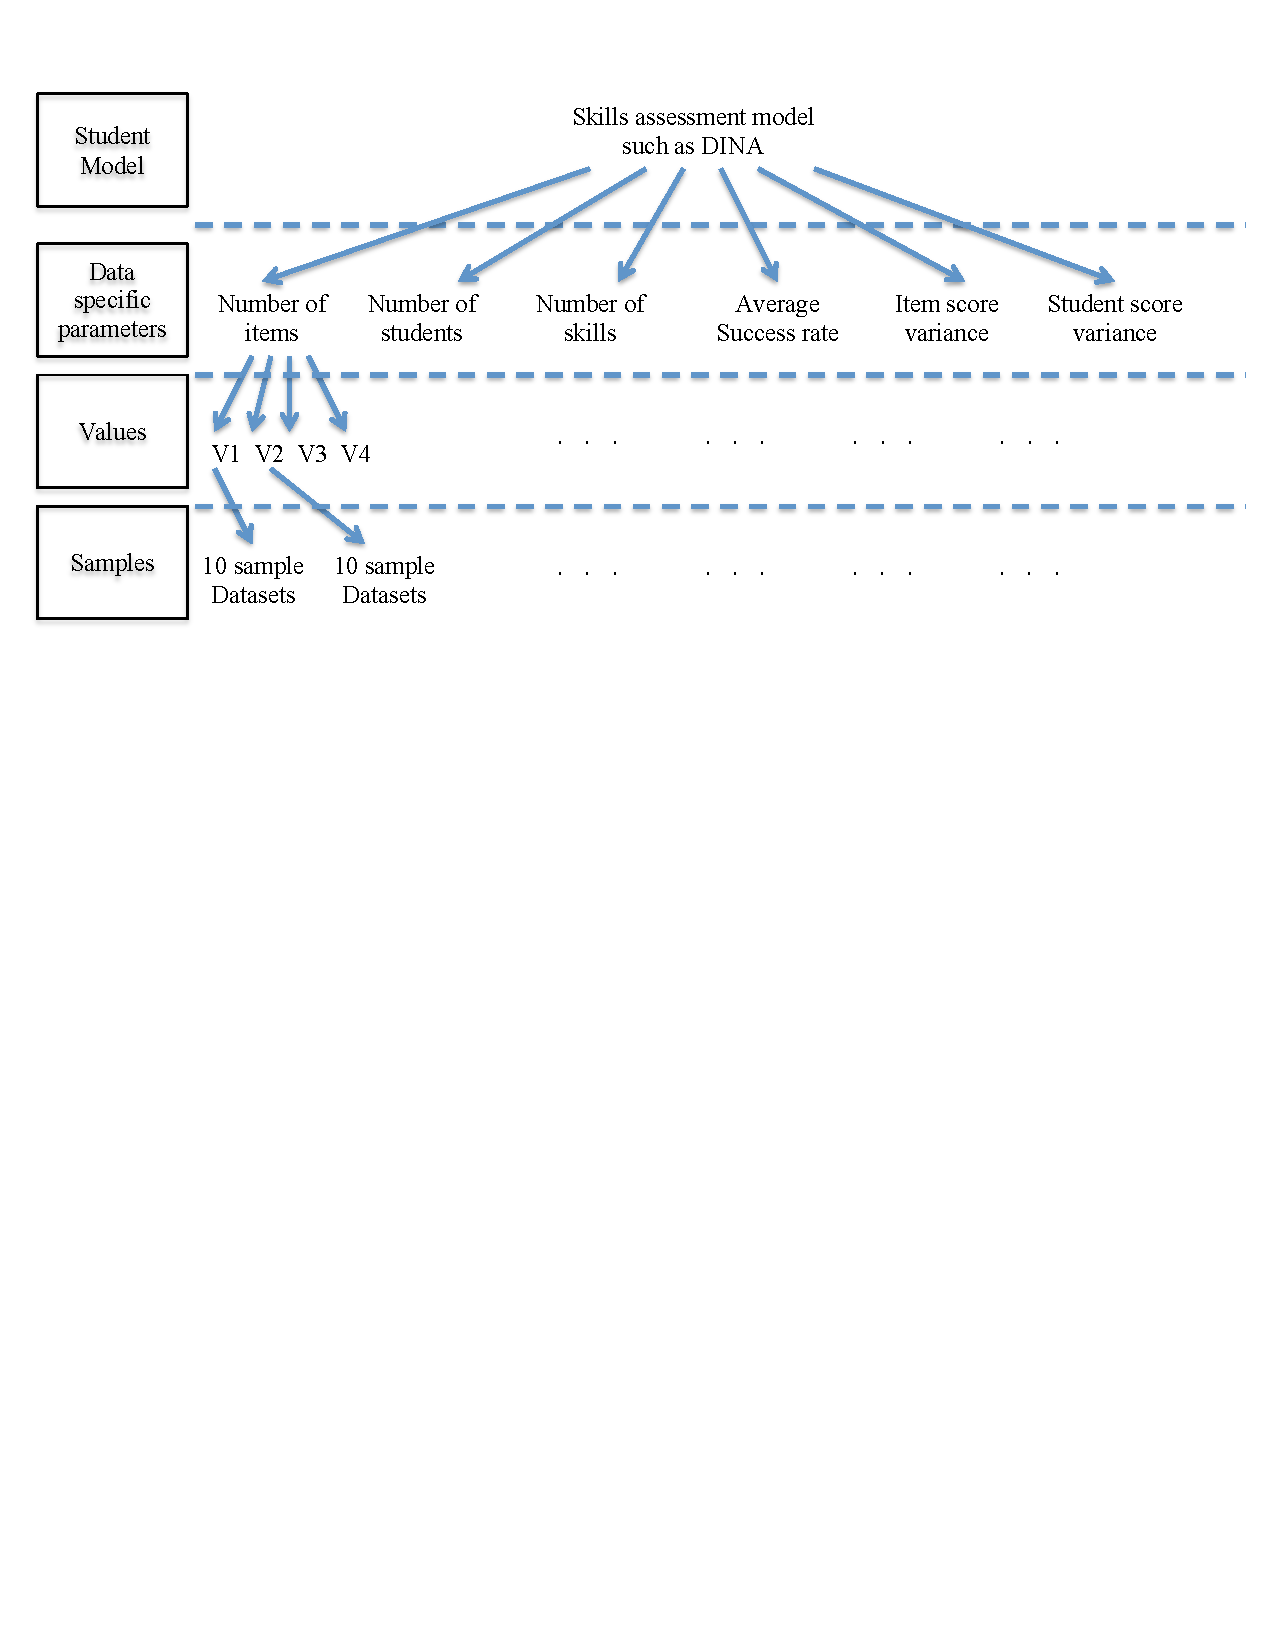
\includegraphics[trim=1cm 17cm 1cm 1cm,scale=0.55]{images/Data-Gen-Break-Down.pdf}
\begin{overprint}
\onslide<1> \small There exists 6 skills assessment models 
\onslide<2> \small There exists 6 skills assessment models X 6 data characteristic parameters 
\onslide<3> \small There exists 6 skills assessment models X 6 data characteristic parameters X 4 values 
\onslide<4> \small There exists 6 skills assessment models X 6 data characteristic parameters X 4 values X 10 samples = 1440 samples in the Database ($DB$)
\onslide<5> $|DB| = 1440$ and $|DC| = 24$
\end{overprint}
\end{frame}

\begin{frame}\frametitle{Prototype definition}
\small{Target performance vector:} $\mathcal{T}^{(tm)} = Performance.vector(D_c^{(tm)} \in DB)$ where: $D_c^{(tm)}$ is characterized with data parameter condition $c \in DC$ and ground truth $(tm)$  \pause
\begin{itemize}
\item Given $c \in DC$ and $m \in \mathcal{M}$ : $D = \{\forall D_i^{(j)} \in DB | i = c , j = m\}$
\item $\mathcal{N}^m$ is a centroid performance prototype defined for model $m$\pause
\item $\mathcal{N}^m = AVG(Performance.vector(D))$ \pause%where in our case  $|D| = 10 | D_c^m \in DB$
\item Pearson correlation coefficient is used as a measure of similarity between $\mathcal{T}^{(tm)}$ and $\mathcal{N}^m$ (for data condition $c$) \pause
\item Next slid shows the average of correlation between $\mathcal{T}^{(tm)}$ and $\mathcal{N}^m$ for all data parameter conditions in $DC$
\end{itemize}
\end{frame}

%Synthetic performance vectors %characteristics
\begin{frame}\frametitle{Degree of similarity between six synthetic performance vector based on the correlation}
\resizebox{\columnwidth}{!}{\begin{tabular}{cc|c|c|c|c|c|c|c|}
&\multicolumn{2}{c}{} & \multicolumn{6}{c}{Target performance vectors} \tabularnewline
&\multicolumn{8}{c}{} \tabularnewline
\cline{4-9} 
&\multicolumn{2}{c|}{} & POKS & IRT & NMF Conj. & DINA & NMF Add. & DINO\tabularnewline
\cline{3-9}
\cline{3-4}
&&POKS & \textbf {0.96} & \multicolumn{1}{|c}{} & \multicolumn{1}{c}{} & \multicolumn{1}{c}{} & \multicolumn{1}{c}{}\tabularnewline
\cline{3-5}
&&IRT & 0.86 & \textbf {0.96} & \multicolumn{1}{|c}{} & \multicolumn{1}{c}{} & \multicolumn{1}{c}{} & \multicolumn{1}{c}{}\tabularnewline
\cline{3-6}
&&NMF Conj. & 0.22 & -0.20 & \textbf {0.96} & \multicolumn{1}{|c}{} & \multicolumn{1}{c}{} & \multicolumn{1}{c}{}\tabularnewline
\cline{3-7}
&&DINA & 0.02 & -0.40 & 0.94 & \textbf {0.96} & \multicolumn{1}{|c}{} & \multicolumn{1}{c}{}\tabularnewline
\cline{3-8}
&&NMF Add. & 0.44 & 0.75 & -0.62 & -0.73 & \textbf {0.93} & \multicolumn{1}{|c}{}\tabularnewline
\cline{3-9}
\multicolumn{1}{c}{\multirow{-6}{*}{\begin{sideways}\small Centroid synthetic\end{sideways}}}&\multicolumn{1}{c|}{\multirow{-6}{*}{\begin{sideways} \small performance vectors\end{sideways}}}&DINO & -0.15 & 0.20 & -0.70 & -0.69 & 0.63 & \textbf {0.95}\tabularnewline
\cline{3-9}
&\multicolumn{1}{c}{} &\multicolumn{1}{c}{} & \multicolumn{1}{c}{} & \multicolumn{1}{c}{} &\multicolumn{1}{c}{} & \multicolumn{1}{c}{} & \multicolumn{1}{c}{} & \multicolumn{1}{c}{}\tabularnewline
\end{tabular}} 
\begin{overprint}
\onslide<1>
\begin{itemize}
	  \item The diagonal shows high correlations because it compares performance vectors of the same model generated datasets. 
	   \item Performance vectors with similar ground truth also show a high correlation. 
\end{itemize}
\onslide<2> In general, correlation similarity provides a very good measure of model fit.
\end{overprint}
\end{frame}


\begin{frame}\frametitle{Degree of similarity between six real datasets and the ground truth based on the correlation}
\resizebox{\columnwidth}{!}{\begin{tabular}{cc|c|c|c|c|c|c|c|c|}

\multicolumn{3}{c}{}&\multicolumn{7}{c}{Target performance vectors of Real Datasets}\tabularnewline   
\multicolumn{9}{c}{}\tabularnewline   
\cline{7-10}
\multicolumn{6}{c|}{}&\multicolumn{4}{c|}{Fraction subsets}   \tabularnewline   
\cline{4-10} 
\multicolumn{3}{c|}{}   & Vomlel &ECPE &Fraction &1&21&22&23\tabularnewline
\cline{3-10}
\cline{3-10}
&&Random & 0.58 &\textbf {0.73} & 0.61   & 0.43 & 0.24 & 0.61 & 0.57 \tabularnewline
\cline{3-10}
&&IRT & \textbf {0.90} & 0.42 & 0.72   & 0.88 & 0.60 & 0.77 & 0.61 \tabularnewline
\cline{3-10}
&&DINA & -0.38  & -0.09 &   0.23 &   0.30 & 0.56 & 0.06 & 0.38 \tabularnewline
\cline{3-10}
&&DINO & 0.34 & 0.15  &  -0.18 &  -0.31 & 0.10 & -0.08 & 0.38 \tabularnewline
\cline{3-10}
&&POKS & 0.75 &0.40  &  \textbf {0.83}  &  \textbf {0.95} &\textbf {0.70} & \textbf {0.83} & \textbf {0.80}\tabularnewline
\cline{3-10}
 &&NMF Conj. & -0.05 & 0.54  & 0.51   & 0.55  & 0.66 & 0.33 & 0.57\tabularnewline
\cline{3-10}
\multicolumn{1}{c}{\multirow{-7}{*}{\begin{sideways} \small Performance Prototype\end{sideways}}}&\multicolumn{1}{c|}{\multirow{-7}{*}{\begin{sideways}of Synthetic Datasets\end{sideways}}}&NMF Add. & 0.39 &0.06   & -0.04   & -0.19 & -0.03 & 0.13 & 0.28\tabularnewline
\cline{3-10}
 \multicolumn{2}{c}{}&\multicolumn{1}{c}{} &\multicolumn{1}{c}{} & \multicolumn{1}{c}{} & \multicolumn{1}{c}{}   & \multicolumn{1}{c}{}  & \multicolumn{1}{c}{} & \multicolumn{1}{c}{} & \multicolumn{1}{c}{} \tabularnewline
\end{tabular}
}
\begin{overprint}
	  \onslide<1> The centroid performance vector of each model is the average of performance vectors of 10 generated datasets
      \onslide<2> Vomlel dataset shows a high correlation with IRT model
      \onslide<3> Fraction with its subset datasets show similarity with POKS model. 
      \onslide<4> As expected, ECPE has the highest correlation with random generated dataset. 
\end{overprint}
\end{frame}

\subsection{Experiment 4: Signature vs. best performer}
\begin{frame}\frametitle{Research questions}
\begin{enumerate}
\item \checkmark What is the \textit{performance vector} of student skills assessment models over real and over synthetic data created using the same models?
\begin{itemize}
\item Experiment 1: Predictive performance of models over real and synthetic data sets
\end{itemize}
\item \checkmark Is the \textit{performance vector} unique to each synthetic data type (data from the same ground truth model)?
\begin{itemize}
\item Experiment 2: Sensitivity of the Model performance over different data generation parameters
\end{itemize}
\item \checkmark Can the \textit{performance vector} be used to define a method to reliably identify the ground truth behind the synthetic data?
\begin{itemize}
\item Experiment 3: Model selection based on performance vector classification
\end{itemize}
\item \textbf{How does the method compare with the standard practice of using the model with the best performance?}
\begin{itemize}
\item Experiment 4: Signature vs. best performer classification
\end{itemize}
\end{enumerate}
\end{frame}

\begin{frame}\frametitle{Problem specification}
\begin{overprint}
\onslide<1> 
\begin{itemize}
	\item What we did? to evaluate the ability of the Signature approach to identify the ground truth model
	\end{itemize}
	\onslide<2> 
	\begin{itemize}
	\item What we did? to evaluate the ability of the Signature approach to identify the ground truth model
	\item What we want to do? to compare the results of classification based on signature approach with the best performer \small approach.
\end{itemize}
	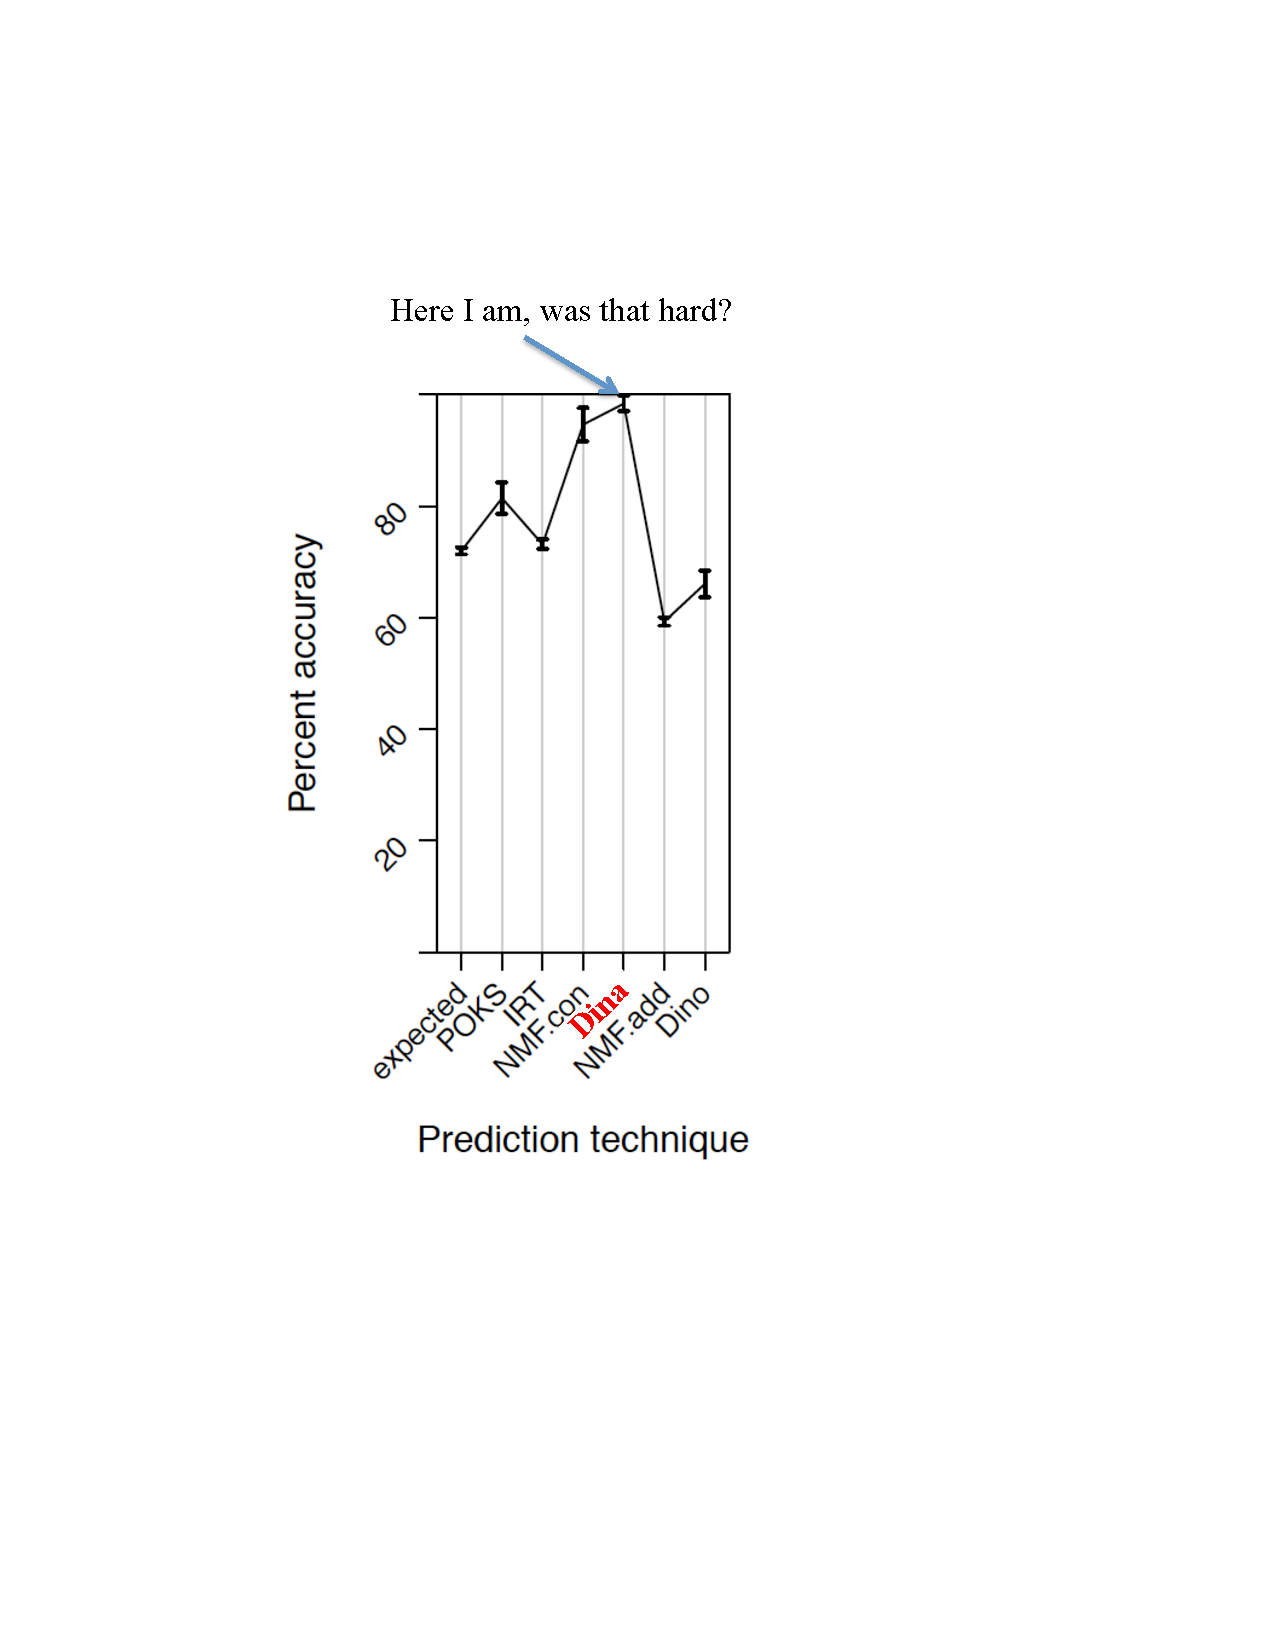
\includegraphics[trim=3cm 10cm 5cm 5cm,scale=0.37]{images/BestPerformer.pdf}
\onslide<3>
\begin{itemize}
	\item What we did? to evaluate the ability of the Signature approach to identify the ground truth model
	\item What we want to do? to compare the results of classification based on signature approach with the best performer \small approach.
	\item Reporting the accuracy of these classification in terms of F1 and accuracy measures
\end{itemize}
\begin{columns}
\begin{column}{.4\textwidth}
\vspace{-0.5cm}
\begin{center}
\resizebox{\columnwidth}{!}{\begin{tabular}{c|c|c|c|}
\multicolumn{2}{c}{}&\multicolumn{2}{c}{Prediction outcome}\tabularnewline
\cline{3-4}
\multicolumn{2}{c|}{}& \multicolumn{1}{c|}{Positive} & \multicolumn{1}{c|}{Negative} \tabularnewline
\cline{2-4}
Actual&  \multicolumn{1}{c|}{Positive }&TP&FN\tabularnewline
\cline{2-4}
value& \multicolumn{1}{c|}{Negative} &FP&TN\tabularnewline
\cline{2-4}
\end{tabular}}

\[Precision = \frac{TP}{TP+FP}\]
\[Recall = \frac{TP}{TP+FN}\]

\end{center}
\end{column}
\begin{column}{.6\textwidth}
\vspace{-1cm}
\begin{center}
\[Accuracy = \frac{TP+TN}{TP+TN+FP+FN}\]
\[F_1 = \frac{Precision.Recall}{Precision+Recall}\]
\end{center}
\end{column}
\end{columns}
\end{overprint}


\end{frame}

\begin{frame}\frametitle{Signature classifier}
\small{Target performance vector:} $\mathcal{T}^{(tm)} = Performance.vector(D_c^{(tm)} \in DB)$ where: $D_c^{(tm)}$ is characterized with data parameter condition $c \in DC$ and ground truth $(tm)$  \pause
\begin{itemize}
\item Given $c \in DC$  : $D = \{\forall D_i^{(j)} \in DB | i = c , j \in \mathcal{M} \}$ \pause
\item Neighbors of $\mathcal{T}^{(tm)}$ are performance vectors of $D$ \pause
\item A majority voting among the ground truth of 10 nearest neighbors to $\mathcal{T}^{(tm)}$ defines the estimated ground truth 
\end{itemize}
\end{frame}


\begin{frame}\frametitle{Results of signature vs. best performer classification}

\resizebox{0.8\columnwidth}{2cm}{\begin{tabular}{c|c|c|c!{\VRule[2pt]}c|c|}
\multicolumn{2}{c}{}&\multicolumn{4}{c}{Performance}\tabularnewline
\cline{3-6}
\multicolumn{2}{c|}{}&\multicolumn{2}{c|}{Best Performer}&\multicolumn{2}{c|}{Signature approach}\tabularnewline
\cline{3-6}
\multicolumn{2}{c|}{}&\multicolumn{1}{c|}{\scriptsize F-Measure}&\scriptsize Accuracy&\scriptsize F-Measure&\scriptsize Accuracy\tabularnewline
\cline{2-6}
&POKS&0.719&0.871&\cellcolor{gray!25}0.998&\cellcolor{gray!25}99.9\tabularnewline
\cline{2-6}
&IRT&0.625&0.908&\cellcolor{gray!25}0.998&\cellcolor{gray!25}99.9\tabularnewline
\cline{2-6}
&NMF Conj.&0.502&0.887&\cellcolor{gray!25}0.985&\cellcolor{gray!25}99.5\tabularnewline
\cline{2-6}
&DINA&0.734&0.891&\cellcolor{gray!25}1&\cellcolor{gray!25}100\tabularnewline
\cline{2-6}
&NMF Add.&0.905&0.969&\cellcolor{gray!25}1&\cellcolor{gray!25}100\tabularnewline
\cline{2-6}
\multicolumn{1}{c|}{\multirow{-7}{*}{\begin{sideways}Models\end{sideways}}}&DINO&0.963&0.988&\cellcolor{gray!25}0.970&\cellcolor{gray!25}0.990\tabularnewline
\cline{1-6}
\multicolumn{2}{|c|}{Total accuracy}&\multicolumn{2}{c|}{75\%}&\multicolumn{2}{c|}{\cellcolor{gray!25}99\%}\tabularnewline
\cline{1-6}
\end{tabular}}
\begin{itemize}
\item The F-measure increases when the signature approach is used for classification.\pause
\item In terms of individual scores per method, the accuracy increases when signature approach is used.\pause
\item The total accuracy considers true positive numbers over number of datasets regardless of individual models
\end{itemize}
\end{frame}

\section{Conclusion}
\subsection{Conclusion and discussion}
\begin{frame}\frametitle{Research questions}
\vspace{-0.5cm}
\begin{overprint}
\onslide<1>
\begin{enumerate}
\item \checkmark What is the \textit{performance vector} of student skills assessment models over real and over synthetic data created using the same models?
\end{enumerate}
\begin{itemize}
\item Experiment 1: Predictive performance of models over real and synthetic data sets
\item In terms of signature pattern : it is unique for each generative model
\item In terms of data points in the performance vector space : They are data points in this space%data points with same ground truth belong to a specific sub-space
\item For real data sets, the performances are not better than the expected performance
\item For synthetic  data, datasets with different ground truths that share some concepts, show a high correlation.
\end{itemize}
\onslide<2>
\begin{enumerate}
\item \begin{scriptsize}
\checkmark Predictive performance of models over real and synthetic data sets
\end{scriptsize} 
\item \checkmark Is the \textit{performance vector} unique to each synthetic data type (data from the same ground truth model)?
\end{enumerate}
\begin{itemize}
\item Experiment 2: Sensitivity of the Model performance over different data generation parameters
\item Different parameters can create different points in the performance vector space
\item There would be a cloud of points for a particular model (Ground truth)
\item The cloud is not too dispersed
\end{itemize}
\onslide<3>
\begin{enumerate}
\item \begin{scriptsize}
\checkmark Predictive performance of models over real and synthetic data sets
\end{scriptsize} 
\item \begin{scriptsize}
\checkmark Sensitivity of the Model performance over different data parameters
\end{scriptsize}  
\item \checkmark Can the \textit{performance vector} be used to define a method to reliably identify the ground truth behind the synthetic data?
\end{enumerate}
\begin{itemize}
\item Experiment 3: Model selection based on performance vector classification
\item A comparison between the target and the prototype signature 
\item Datasets that share a common source have correlated performance vectors.
\end{itemize}
\onslide<4>
\begin{enumerate}
\item \begin{scriptsize}
\checkmark Predictive performance of models over real and synthetic data sets
\end{scriptsize} 
\item \begin{scriptsize}
\checkmark Sensitivity of the Model performance over different data parameters
\end{scriptsize}  
\item \begin{scriptsize}
\checkmark Model selection based on performance vector classification
\end{scriptsize} 
\item \checkmark How does the method compare with the standard practice of using the model with the best performance?
\end{enumerate}
\begin{itemize}
\item Experiment 4: Signature vs. best performer classification
\item The ground truth model does not always correspond to the best performer and our approach provides a more reliable means
%conclusion
\end{itemize}

\end{overprint}
\end{frame}


%\begin{frame}\frametitle{Conclusion}
%\begin{itemize}
%\item Model fit of a data set is defined as the similarity between \textit{prototype} and \textit{target} performance vector \pause
%\item The ground truth model does not always correspond to the best performer and our approach provides a more reliable means \pause
%This means of determining a data set’s ground truth is made possible because the synthetic data sets have very distinct performance patterns, showing sharp differences across models. and uniqueness characteristics
%\item Datasets that share a common source have correlated performance vectors. \pause % Fraction data
%\item It does not seem to substantially extend to data that shares the same domain
%\end{itemize}
%\end{frame}

%\begin{frame}\frametitle{Conclusion}
%\begin{itemize}
%\item For real data sets, the performances are not better than the expected performance \pause %the conclusion behind that can be either the ground truth is not among the candidate models, or the best performer is not necessarily the ground truth.
%\item For synthetic  data, datasets with different ground truths that share some concepts, show a high correlation. \pause
%\item \textit{performance vector} changes for some data specific parameters but it still shows a high correlation with datasets with the same ground truth. \pause
%\item Best performer may not be the model that is most representative of the ground truth.
%\end{itemize}
%\end{frame}

\subsection{Future works}
\begin{frame}\frametitle{Future works}
\begin{itemize}
\item to be extend over different models, different domains and more datasets \pause
\item generalize to dynamic data and skills assessment models \pause
\item Candidate models and their complexity where the data is created with a mixture of models \pause
\item Application in other fields of study  
\end{itemize}
\end{frame}
\subsection{Questions}
\begin{frame}\frametitle{Thank you}
\begin{figure}

\includegraphics[scale =0.55] {images/Question} 
\end{figure}
\end{frame}
\end{document}

%Pardos Work compared with our work : make link between performance space and parameter space.  We look for close points of synthetic data, they look for similar likelihood surfaces in the space of parameters
